% ===========================================================================
% Batcher.  Author: Stephen Offer.
%
% Builds with stock TeX Live (`make`). Two-column, 10pt, conference formatting.
% To retarget a venue, drop in its .sty at the STYLE lines below.
% ===========================================================================

\documentclass[10pt,twocolumn,letterpaper]{article}   % STYLE

\usepackage[margin=0.7in]{geometry}                  % STYLE: a venue style sets its own
\usepackage[T1]{fontenc}
\usepackage[utf8]{inputenc}
\usepackage{times}
\usepackage{amsmath,amssymb}
\usepackage{booktabs}
\usepackage{array}
\usepackage{colortbl}
\usepackage{graphicx}
\usepackage{tikz}
\usepackage{pgfplots}
\pgfplotsset{compat=1.16}
\usepackage{balance}
\usepackage[hidelinks,pdfusetitle]{hyperref}
\hypersetup{
  pdftitle={Batcher: Declared Execution Contracts Across Cores, Clusters, Streams, and Models},
  pdfauthor={Stephen Offer},
  pdfsubject={Data engine architecture: mergeable, partitioned and replicated operator contracts},
  pdfkeywords={query processing, distributed execution, streaming, mergeable aggregation,
               Apache Arrow, adaptive optimization, model inference},
  pdflang={en-US},
}
\usepackage[capitalize,noabbrev]{cleveref}
\usepackage{microtype}
\usepackage[numbers,sort&compress]{natbib}
\usepackage[skip=3pt,font=small]{caption}
\usepackage{placeins}

\usepackage{float}
\usepackage{listings}
\lstset{
  basicstyle=\ttfamily\scriptsize, columns=fullflexible, keepspaces=true,
  language=Python, showstringspaces=false,
  keywordstyle=\color{okBlue}\bfseries, stringstyle=\color{okGreen},
  commentstyle=\itshape\color{pfigGray}, aboveskip=2pt, belowskip=0pt,
  xleftmargin=2pt, frame=none, numbers=none,
}

% ---------------------------------------------------------------------------
% Shared TikZ styles for paper figures.
%
% Drop this in the preamble, then draw every diagram with these styles. One edit
% here restyles every figure in the paper, which is the whole point: consistency
% across figures is what makes a paper look professionally produced.
%
% Colors are the Okabe-Ito colorblind-safe palette. Meaning is never carried by
% color alone: use `pfig/box` for context and `pfig/new` for what the paper
% contributes, and the contrast survives a grayscale print.
%
% Requires: \usepackage{tikz} and the libraries loaded below. Builds with stock
% TeX Live, no external binaries.
% ---------------------------------------------------------------------------

\usetikzlibrary{arrows.meta,positioning,fit,backgrounds,calc,shapes.geometric}

% Okabe-Ito palette ---------------------------------------------------------
\definecolor{okBlue}{HTML}{0072B2}
\definecolor{okSky}{HTML}{56B4E9}
\definecolor{okGreen}{HTML}{009E73}
\definecolor{okOrange}{HTML}{E69F00}
\definecolor{okVermillion}{HTML}{D55E00}
\definecolor{okPurple}{HTML}{CC79A7}
\definecolor{okYellow}{HTML}{F0E442}
\definecolor{pfigGray}{HTML}{6E6E6E}
\definecolor{pfigLight}{HTML}{EDEDED}

\tikzset{
  % Base node: context components. Deliberately quiet.
  pfig/box/.style={
    draw=pfigGray, fill=white, line width=0.6pt,
    rounded corners=2pt, inner sep=4pt, align=center,
    font=\footnotesize, minimum height=7mm, text=black
  },
  % The contribution. One accent, used sparingly: if everything is emphasized,
  % nothing is.
  pfig/new/.style={
    pfig/box, draw=okBlue, fill=okSky!18, line width=1pt, font=\footnotesize\bfseries
  },
  % Secondary emphasis, when a second component genuinely needs to stand out.
  pfig/alt/.style={
    pfig/box, draw=okOrange, fill=okOrange!12, line width=0.9pt
  },
  % External input or user.
  pfig/io/.style={
    pfig/box, rounded corners=6pt, fill=pfigLight, draw=pfigGray
  },
  % Data store.
  pfig/store/.style={
    pfig/box, cylinder, shape border rotate=90, aspect=0.25,
    inner sep=3pt, minimum width=16mm
  },
  % Decision or gate.
  pfig/gate/.style={
    pfig/box, diamond, aspect=1.8, inner sep=1pt, minimum height=6mm
  },
  % Swimlane or grouping background.
  pfig/lane/.style={
    draw=pfigGray!50, dashed, line width=0.5pt, rounded corners=3pt,
    fill=pfigLight!45, inner sep=5pt
  },
  % Arrows. Solid for the main path, dashed for feedback or optional flow.
  pfig/arrow/.style={
    -{Stealth[length=2.4mm,width=1.6mm]}, line width=0.7pt, draw=black
  },
  pfig/arrowD/.style={
    pfig/arrow, dashed, draw=pfigGray
  },
  pfig/arrowNew/.style={
    pfig/arrow, draw=okBlue, line width=0.9pt
  },
  % Edge labels: small, never smaller than 7pt at final size.
  pfig/label/.style={
    font=\scriptsize, text=black, inner sep=1.5pt, fill=white, fill opacity=0.85,
    text opacity=1
  },
  % Section caption inside a figure.
  pfig/title/.style={
    font=\footnotesize\bfseries, text=black
  },
}

% ---------------------------------------------------------------------------
% Example. Delete once you have your own figures.
%
% \begin{figure}[t]
%   \centering
%   \begin{tikzpicture}[node distance=6mm and 9mm]
%     \node[pfig/io]  (in)   {Workload};
%     \node[pfig/box, right=of in]  (enc) {Encoder};
%     \node[pfig/new, right=of enc] (ours){Verifier-guided\\memory};
%     \node[pfig/box, right=of ours](dec) {Decoder};
%     \node[pfig/io,  right=of dec] (out) {Answer};
%     \draw[pfig/arrow]    (in)  -- (enc);
%     \draw[pfig/arrowNew] (enc) -- node[pfig/label]{states} (ours);
%     \draw[pfig/arrowNew] (ours)-- (dec);
%     \draw[pfig/arrow]    (dec) -- (out);
%     \draw[pfig/arrowD]   (dec.south) to[out=-90,in=-90] node[pfig/label]{retry} (ours.south);
%   \end{tikzpicture}
%   \caption{...}
% \end{figure}
% ---------------------------------------------------------------------------


\newcommand{\sys}{Batcher}
\newcommand{\kyber}{Kyber}
\newcommand{\carbo}{Carbonite}
\newcommand{\pcf}{\ensuremath{\mathsf{partial}\!\rightarrow\!\mathsf{combine}\!\rightarrow\!\mathsf{finalize}}}
\newcommand{\win}{\cellcolor{okSky!22}}
\newcommand{\loss}{\cellcolor{okOrange!16}}
\newcommand{\Ca}{\textsc{C1}}
\newcommand{\Cb}{\textsc{C2}}
\newcommand{\Cc}{\textsc{C3}}
\newcommand{\E}[1]{\textsf{E#1}}
% The ratio used throughout: Batcher's milliseconds over the baseline's, so
% below 1.00 is a Batcher win. Defined once here and named at every table.
\newcommand{\bx}{\ensuremath{b/x}}

% Float placement: allow a page to carry more float and still take text, rather
% than leaving a column half empty next to a table.
\renewcommand{\topfraction}{0.92}
\renewcommand{\bottomfraction}{0.75}
\renewcommand{\textfraction}{0.06}
\renewcommand{\floatpagefraction}{0.80}
\renewcommand{\dbltopfraction}{0.92}
\renewcommand{\dblfloatpagefraction}{0.80}
\setcounter{topnumber}{3}
\setcounter{bottomnumber}{2}
\setcounter{totalnumber}{5}

\setlength{\abovedisplayskip}{4pt}
\setlength{\belowdisplayskip}{4pt}

\title{\sys{}: Declared Execution Contracts Across\\Cores, Clusters, Streams, and Models}

\author{Stephen Offer\\ \small Anyscale \quad\textbullet\quad \texttt{stephen.offer@anyscale.com}}
\date{}

\begin{document}
\maketitle

\begin{abstract}
\noindent
Data engines usually cross the line between one node and a cluster, or between bounded and
continuous input, by adding an execution path on the far side, and then must keep the paths in
agreement. \sys{} instead admits a stateful operator only if it declares an execution contract,
and its distributed scheduler dispatches on that contract. \textbf{\Ca{}} operators merge
partial states under a commutative monoid. \textbf{\Cb{}} operators run independently on each
partition of a declared hash or range exchange. \textbf{\Cc{}} operators have no partitioning
key: they replicate a bounded input or iterate ordinary plans under a round cap, and refuse
past either budget. A registry classifies every IR operator and aggregate, and the test suite
holds it exhaustive. The micro-batch path and the model-inference operators, which are plan
expressions rather than opaque callbacks, run under the same contracts.
On one 48-core machine reading the same Arrow buffers, \sys{} beats DuckDB on six of six suites
(geometric-mean ratios $0.16$ to $0.83$). Against DuckDB's own compressed store it leads five
($0.35$ to $0.75$) and is at parity on the sixth. At TPC-H sf100 on a 100-worker fleet it leads
Daft on three pipelines by $3.7$ to $109\times$. The latency wins cost CPU ($1.86\times$
DuckDB's on TPC-H sf1), and \sys{} loses the Join Order Benchmark by 11\%.
\end{abstract}

\begin{figure*}[tbp]
\centering
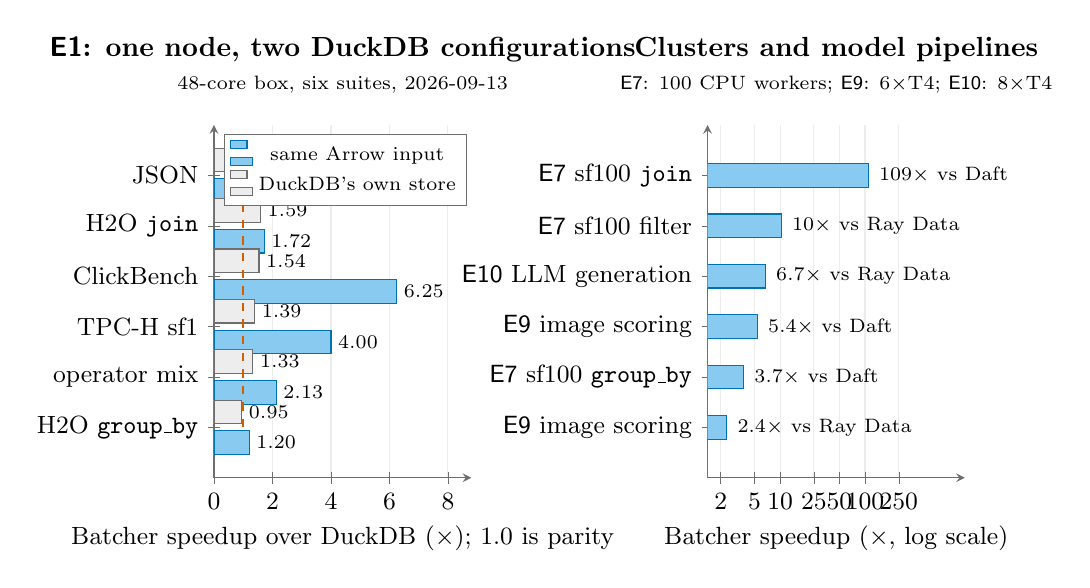
\begin{tikzpicture}
\pgfplotsset{
  hbar/.style={
    xbar, bar width=3.0mm, xbar=0.9mm,
    enlarge y limits=0.02,
    axis lines=left, axis line style={draw=pfigGray},
    xmajorgrids, grid style={pfigLight, line width=0.4pt},
    tick style={draw=pfigGray},
    yticklabel style={font=\small, align=right},
    xticklabel style={font=\small},
    xlabel style={font=\small, yshift=1pt},
    title style={font=\normalsize\bfseries, align=center, yshift=2pt},
    legend style={font=\small, draw=pfigGray, fill=white},
    nodes near coords style={font=\scriptsize, anchor=west, inner sep=2.4pt},
  }
}
% ---- Panel A: single node, two storage configurations -----------------------
\begin{axis}[hbar, name=relA,
  width=0.40\textwidth, y=6.4mm,
  xmin=0, xmax=8.8, xtick={0,2,4,6,8},
  symbolic y coords={padA,gb,ops,tpch,cb,join,json,padB},
  ytick={gb,ops,tpch,cb,join,json},
  yticklabels={H2O \texttt{group\_by},operator mix,TPC-H sf1,ClickBench,H2O \texttt{join},JSON},
  xlabel={\sys{} speedup over DuckDB ($\times$); 1.0 is parity},
  title={\E{1}: one node, two DuckDB configurations\\{\scriptsize\mdseries 48-core box, six suites, 2026-09-13}},
  legend style={at={(0.985,0.975)}, anchor=north east, legend columns=1, row sep=0pt,
                inner sep=2pt, font=\scriptsize},
  nodes near coords={\pgfmathprintnumber[fixed,precision=2,zerofill]{\pgfplotspointmeta}},
]
\addplot[forget plot, draw=none, fill=none, nodes near coords={}]
  coordinates {(0,padA) (0,padB)};
\addplot[draw=okBlue, fill=okSky!70]
  coordinates {(1.20,gb) (2.13,ops) (4.00,tpch) (6.25,cb) (1.72,join) (3.13,json)};
\addlegendentry{same Arrow input}
\addplot[draw=pfigGray, fill=pfigLight]
  coordinates {(0.95,gb) (1.33,ops) (1.39,tpch) (1.54,cb) (1.59,join) (2.86,json)};
\addlegendentry{DuckDB's own store}
\draw[draw=okVermillion, dashed, line width=0.8pt] (axis cs:1,gb) -- (axis cs:1,json);
\end{axis}
% ---- Panel B: cluster and model pipelines -----------------------------------
\begin{axis}[hbar, name=aiB, at={($(relA.east)+(30mm,0)$)}, anchor=west,
  width=0.40\textwidth, y=6.4mm,
  xmode=log, xmin=1.4, xmax=1500, xtick={2,5,10,25,50,100,250},
  xticklabels={2,5,10,25,50,100,250},
  log ticks with fixed point,
  point meta=explicit symbolic,
  symbolic y coords={padA,img2,gb100,img1,llm,fc100,join100,padB},
  ytick={img2,gb100,img1,llm,fc100,join100},
  yticklabels={\E{9} image scoring,\E{7} sf100 \texttt{group\_by},\E{9} image scoring,
               \E{10} LLM generation,\E{7} sf100 filter,\E{7} sf100 \texttt{join}},
  xlabel={\sys{} speedup ($\times$, log scale)},
  title={Clusters and model pipelines\\{\scriptsize\mdseries \E{7}: 100 CPU workers; \E{9}: 6$\times$T4; \E{10}: 8$\times$T4}},
  nodes near coords={\pgfplotspointmeta},
]
\addplot[forget plot, draw=none, fill=none, nodes near coords={}]
  coordinates {(1.5,padA) [{}] (1.5,padB) [{}]};
\addplot[draw=okBlue, fill=okSky!70] coordinates {
  (2.36,img2)  [{\,2.4$\times$ {\scriptsize vs Ray Data}}]
  (3.72,gb100) [{\,3.7$\times$ {\scriptsize vs Daft}}]
  (5.40,img1)  [{\,5.4$\times$ {\scriptsize vs Daft}}]
  (6.71,llm)   [{\,6.7$\times$ {\scriptsize vs Ray Data}}]
  (10.3,fc100) [{\,10$\times$ {\scriptsize vs Ray Data}}]
  (109.0,join100) [{\,109$\times$ {\scriptsize vs Daft}}]};
\end{axis}
\end{tikzpicture}
\caption{Headline results, tagged by experiment; \cref{tab:protocol} binds each tag to its
hardware and date and states the protocol. Left: six suites against DuckDB on one machine,
blue on the identical zero-copy Arrow buffers \sys{} reads, grey after an untimed ingest into
DuckDB's compressed, zone-mapped store. The grey bars pit DuckDB's storage and execution
against \sys{}'s execution alone, and \cref{sec:eval-storage} explains why that isolates
neither. Right: separate experiments on different fleets, on a log axis, not one matched
experiment. Every bar passed a correctness gate before it was timed.}
\label{fig:headline}
\end{figure*}

% ===========================================================================
\section{Introduction}
\label{sec:intro}
% ===========================================================================

Ask a database engineer how \texttt{GROUP BY} works and you often get two answers: a hash
table on one machine, and on a cluster a partial pass followed by a shuffle and reduce. Many
stacks build these as separate operators in a single-node engine and a distributed one, often
beside a stream processor and a model-serving runtime with their own \texttt{GROUP BY} or
notion of a user function. Some systems avoid the split. Flink runs
bounded input as a special case of one streaming runtime~\cite{carbone2015flink}, and the
Dataflow model gives batch and streaming one specification~\cite{akidau2015dataflow}. Spark SQL
sends its local and distributed modes through the same physical
operators~\cite{armbrust2015sparksql}. None of them makes a declared execution contract the
only route by which a stateful operator enters the engine. This paper tests that design.

\sys{}'s own history shows why the route matters. A floating-point grouping key grouped
correctly in the local hash table and split into two groups after a distributed shuffle. The
single-node suite stayed green throughout, since that path was correct. Nothing forced the two
paths to agree.

\subsection{What changed}
\label{sec:shifts}

Most organizations run a distributed stack designed between roughly 2009 and 2014 for
conditions that have since moved. Spark starts from the premise that the data does not
fit in one machine's memory~\cite{zaharia2012rdd}. The single node measured here has 48
hardware threads and 92\,GiB, which is not large, yet a query that takes milliseconds
in-process can take seconds through a distributed runtime's dispatch. Distribution therefore
has to become a property of the query rather than of the engine. Freshness went from nightly
to continuous, so bounded input is no longer the only case an engine plans for. Object storage,
schema drift and opaque operators (a regular expression, a JSON extraction, an embedding
model, an LLM call) took away the curated statistics a static optimizer prices from, which
argues for measuring instead (\cref{sec:learning}). Models moved into
the middle of pipelines. They read decoded media and run on a device, then feed a join on CPU
(\cref{sec:pipeline}). Practitioners write Python, where the usual escape hatch is a user
function the optimizer cannot see into (\cref{sec:interface}). IDC projects that most enterprise
data is unstructured~\cite{idc2018datasphere}, a forecast rather than a census; either way, an
engine whose type system stops at scalars must hand an image or a clip to something else.

\subsection{The admission rule}

\sys{} responds by constraining its operator vocabulary instead of adding an execution layer
per regime. A stateful operator enters only with one of three contracts (\cref{sec:algebra}).
\Ca{} is a mergeable \pcf{} triple. \Cb{} evaluates partition-locally after a declared hash or
range exchange; the range form also needs a total order and a tie policy. \Cc{} covers
operators with no partitioning key at all. Its replicate and iterate forms each carry a
budget, and a breach raises an error instead of falling back to one node. A registry maps
every relational operator and aggregate in the IR to its contract and a declared state class.
Adding an IR tag without an entry fails a unit test.

The contracts form a scheduling interface, not a compactness theorem. \Ca{}
admits \texttt{DISTINCT} and \texttt{array\_agg}, whose state grows with what they retain, and
\cref{tab:vocab} names such operators instead of hiding them behind one state bound. Every
contract does make the partition count a scheduling variable and nothing more. It can reorder
a floating-point sum and, in the four cases SQL leaves open, change which permitted answer
comes back (\cref{sec:equivalence}). The relation itself does not change.

The micro-batch path uses the same vocabulary: a \Ca{} operator folds each trigger's partial
into its running state. Media decode is a plan expression too, as are embedding and model
inference, so \kyber{} (the optimizer) and \carbo{} (the resource manager) reason about them
alongside the joins around them.\footnote{The engine is Apache-2.0 at
\url{https://github.com/stephenoffer/batcher}, as are the benchmark harness and every
comparator adapter. \Cref{sec:appendix-protocol} lists the commands behind every experiment.}

\subsection{Contributions}

\begin{enumerate}\itemsep1pt \parskip0pt \topsep2pt
\item \textbf{Three execution contracts enforced as an admission rule.} Each states a merge
or partitioning law, a state class and a failure mode, and a registry classifies the whole IR
against them (\cref{sec:algebra}). The algebra is old. Enforcing it as the only admission
route is the design choice under test.
\item \textbf{A stated equivalence relation} between execution modes, exact on the relation
except for floating-point reassociation and the four SQL-open choices. Integer \texttt{SUM}
overflow does not depend on the partitioning (\cref{sec:equivalence}).
\item \textbf{Measurement-driven planning under a result-invariance rule}: a stale measurement
costs time and never changes an answer. An ablation shows which part of the repeated-query
speedup it buys (\cref{sec:learning,sec:eval-learning}).
\item \textbf{Relational and model operators in one plan}, under one optimizer and one
resource manager (\cref{sec:interface,sec:pipeline}).
\item \textbf{A traceable evaluation}: every number carries an experiment tag bound to hardware,
date, lineup and statistic (\cref{tab:protocol}). Storage configurations, CPU cost, memoized
answers and worker loss are reported separately (\cref{sec:eval}).
\end{enumerate}

\paragraph{Reading the numbers.}
\label{sec:convention}
A ratio written \bx{} means $\text{\sys{}}_{ms}/x_{ms}$ for baseline $x$, so \textbf{below 1.00
means \sys{} is faster}. Suite ratios are geometric means over the included queries; the bar
charts invert them into speedups. DuckDB runs in the two configurations \cref{fig:headline}
defines, \emph{same Arrow} and \emph{native store}, never netted together.
% ===========================================================================
\section{System overview}
\label{sec:arch-overview}
% ===========================================================================

\sys{} puts a Python control plane over a Rust data plane. Arrow
\texttt{RecordBatch}~\cite{arrow} is the only columnar format, at every internal boundary and
across the FFI (\cref{fig:arch}). Python builds a lazy plan, optimizes it and lowers it to a
JSON IR. The Rust engine executes the IR and returns Arrow batches through the C Data
Interface. The control plane pays per query, so its seven optimizer phases fit in
single-digit milliseconds (\cref{sec:smallquery}). The data plane pays per row.

\begin{figure*}[tbp]
\centering
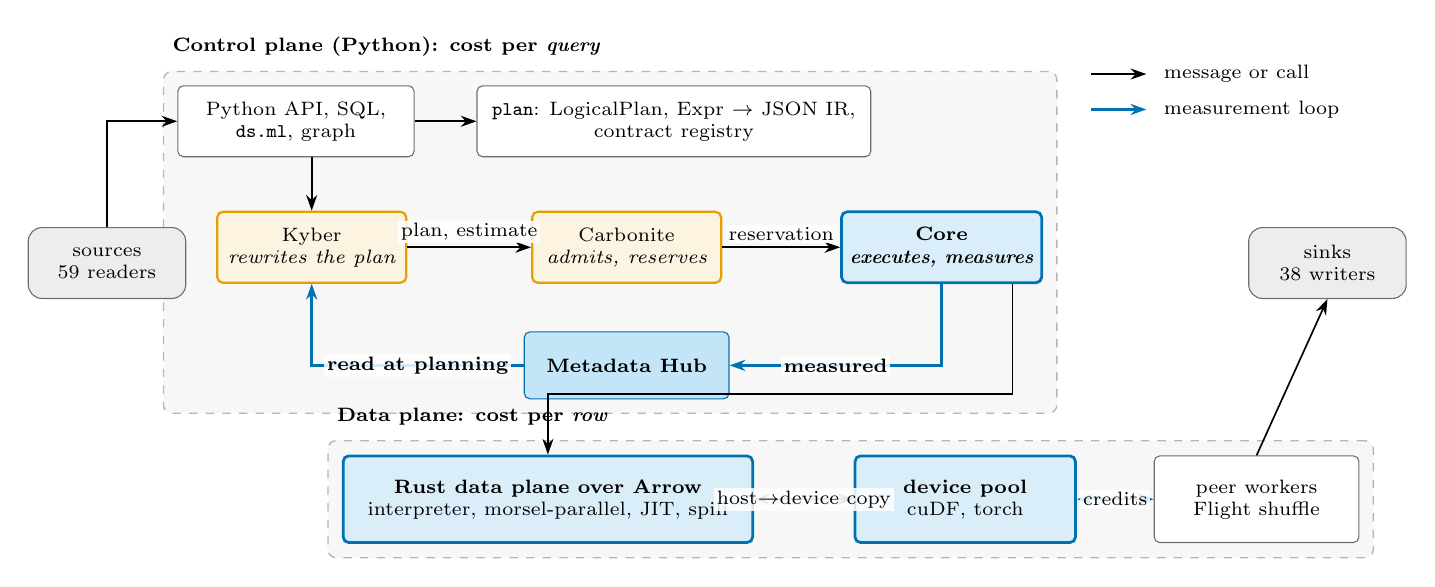
\begin{tikzpicture}[x=1mm,y=1mm,
  comp/.style={draw=pfigGray, fill=white, rounded corners=2pt, inner sep=3pt,
               font=\scriptsize, align=center, minimum height=9mm, minimum width=24mm},
  sub/.style={comp, draw=okOrange, fill=okOrange!12, line width=0.8pt},
  core/.style={comp, draw=okBlue, fill=okSky!22, line width=1pt, font=\scriptsize\bfseries},
  hub/.style={comp, draw=okBlue, fill=okSky!35, minimum width=26mm, minimum height=8.5mm,
              font=\scriptsize\bfseries},
  io/.style={comp, fill=pfigLight, rounded corners=5pt, minimum width=20mm},
  msg/.style={-{Stealth[length=2.0mm,width=1.4mm]}, draw=black, line width=0.6pt},
  loop/.style={-{Stealth[length=2.0mm,width=1.4mm]}, draw=okBlue, line width=1.1pt},
  lbl/.style={font=\scriptsize, inner sep=1pt, fill=white, fill opacity=0.85, text opacity=1}]

  \node[io] (src) at (2,22) {sources\\ \scriptsize 59 readers};
  \node[io] (snk) at (157,22) {sinks\\ \scriptsize 38 writers};

  \node[comp, minimum width=30mm] (api) at (26,40) {Python API, SQL,\\\texttt{ds.ml}, graph};
  \node[comp, minimum width=50mm] (plan) at (74,40)
       {\texttt{plan}: LogicalPlan, Expr $\rightarrow$ JSON IR,\\contract registry};
  \node[sub]  (ky) at (28,24) {\kyber{}\\{\scriptsize\itshape rewrites the plan}};
  \node[sub]  (ca) at (68,24) {\carbo{}\\{\scriptsize\itshape admits, reserves}};
  \node[core] (co) at (108,24) {Core\\{\scriptsize\itshape executes, measures}};
  \node[hub]  (mh) at (68,9) {Metadata Hub};

  \node[core, minimum width=52mm, minimum height=11mm] (rust) at (58,-8)
       {Rust data plane over Arrow\\{\scriptsize\mdseries interpreter, morsel-parallel, JIT, spill}};
  \node[core, minimum width=28mm, minimum height=11mm] (dev) at (111,-8)
       {device pool\\{\scriptsize\mdseries cuDF, torch}};
  \node[comp, minimum width=26mm, minimum height=11mm] (net) at (148,-8)
       {peer workers\\{\scriptsize Flight shuffle}};

  \draw[msg] (src) |- (api.west);
  \draw[msg] (api) -- (plan);
  \draw[msg] (plan.south -| ky.north) -- (ky.north);
  \draw[msg] (ky) -- node[lbl,above=0.4mm]{plan, estimate} (ca);
  \draw[msg] (ca) -- node[lbl,above=0.4mm]{reservation} (co);
  \draw[loop] (co.south) |- node[lbl, pos=0.75]{\bfseries measured} (mh.east);
  \draw[loop] (mh.west) -| node[lbl, pos=0.25]{\bfseries read at planning} (ky.south);
  \draw[msg] ($(co.south)+(9,0)$) -- ++(0,-14) -| (rust.north);
  \draw[{Stealth[length=2.0mm,width=1.4mm]}-{Stealth[length=2.0mm,width=1.4mm]},
        draw=pfigGray, line width=0.9pt] (rust.east) -- node[lbl]{host$\rightarrow$device copy} (dev.west);
  \draw[{Stealth[length=2.0mm,width=1.4mm]}-{Stealth[length=2.0mm,width=1.4mm]},
        draw=okBlue, line width=0.9pt] (dev.east) -- node[lbl]{credits} (net.west);
  \draw[msg] (net.north) -- (snk.south);

  \begin{scope}[on background layer]
    \node[pfig/lane, fit=(api)(plan)(ky)(ca)(co)(mh),
      label={[pfig/title,anchor=south west,yshift=0.6mm]north west:\scriptsize Control plane (Python): cost per \emph{query}}] {};
    \node[pfig/lane, fit=(rust)(dev)(net),
      label={[pfig/title,anchor=south west,yshift=0.6mm]north west:\scriptsize Data plane: cost per \emph{row}}] {};
  \end{scope}
  \draw[msg] (127,46) -- ++(7,0); \node[font=\scriptsize, anchor=west] at (135,46) {message or call};
  \draw[loop] (127,41.5) -- ++(7,0); \node[font=\scriptsize, anchor=west] at (135,41.5) {measurement loop};
\end{tikzpicture}
\caption{The whole engine. Arrows show messages and data flow, not source imports; a lint
contract checks on every commit that \kyber{}, \carbo{} and Core never import one another.
Relational and expression work runs in Rust over Arrow and returns through the Arrow C Data
Interface, a pointer exchange inside one process. Three parts of the data plane are not Rust:
a user's batch callback, a model framework's own code, and the cuDF device tier, which copies
its inputs from host to device memory. The peer-worker edge crosses a network, with framing and
real copies. Measurements reach planning only through the Metadata Hub.}
\label{fig:arch}
\end{figure*}

\paragraph{The API surface.} Users meet \sys{} at four layers, and SQL included, all of them
lower to the same \texttt{LogicalPlan} (\cref{tab:api}). A \texttt{Dataset}, the lazy and
immutable handle to a plan, has 153 public members, from relational verbs and windows to
terminals such as \texttt{collect}, \texttt{iter\_batches} and \texttt{write}. The scalar
language, \texttt{Expr}, has 191 methods and eleven accessor namespaces (\texttt{.str} alone
has 186). Feature surfaces sit on top: \texttt{ds.ml} for models, \texttt{bt.graph} for graph
analytics over an edge table, \texttt{ds.dq} for data-quality contracts, and a security
catalog whose row filters and column masks are plan rewrites. Streaming needs no separate API.
Give a sink a \texttt{trigger}, \texttt{output\_mode} or \texttt{checkpoint} and the same plan
runs continuously.

\begin{table}[tbp]
\centering\scriptsize
\setlength{\tabcolsep}{2.4pt}
\begin{tabular}{@{}>{\raggedright\arraybackslash}p{0.19\columnwidth}>{\raggedright\arraybackslash}p{0.77\columnwidth}@{}}
\toprule
Layer & What it contains \\
\midrule
Entry points & \texttt{bt.read.*} (59 readers: files, media, genomics, lakehouse tables, 11 databases, 9 stream sources); \texttt{from\_pandas}/\texttt{polars}/\texttt{arrow}/\texttt{torch} and 20 other constructors; \texttt{bt.sql}, \texttt{Session} \\
\addlinespace[1pt]
\texttt{Dataset} & select, filter, \texttt{with\_columns}, join (equi, as-of, inequality, lookup), \texttt{group\_by}/\texttt{agg}, cube/rollup, set operations, sort, top-$k$, pivot/unpivot, explode, windows, \texttt{map\_batches}; 38 \texttt{ds.write.*} sinks incl.\ Delta, Iceberg and \texttt{merge\_into} \\
\addlinespace[1pt]
\texttt{Expr} & 191 methods; namespaces \texttt{.str .list .dt .json .map .struct .seq .meta} and the media namespaces \texttt{.image .audio .video}; 672 top-level names incl.\ geospatial \texttt{st\_*} and rigid-body \texttt{quat\_*}/\texttt{se3\_*} \\
\addlinespace[1pt]
Feature surfaces & \texttt{ds.ml} (\texttt{infer}, \texttt{embed}, \texttt{generate}, \texttt{iter\_torch\_batches}, similarity join); \texttt{bt.graph} (60 algorithms); \texttt{ds.dq}; \texttt{ds.scd} and CDC; governance and lineage \\
\addlinespace[1pt]
Streaming & a sink with \texttt{trigger}/\texttt{checkpoint}; \texttt{with\_watermark}, \texttt{session\_window}, \texttt{join\_stream}, \texttt{transform\_with\_state} \\
\addlinespace[1pt]
Operations & \texttt{Config} (15 sections), \texttt{config\_context}; \texttt{start\_ui}, query history, cancellation; 17 typed errors rooted at \texttt{BatcherError} \\
\bottomrule
\end{tabular}
\caption{The public API by layer, as counted in the installed package. All of it lowers to
one \texttt{LogicalPlan} and one JSON IR.}
\label{tab:api}
\end{table}

\paragraph{The Python packages.} An import-linter contract enforces the control plane's
layering on every commit. Only \texttt{api} imports the four subsystems, which
it sequences at a terminal call. \kyber{} rewrites plans and never executes. \carbo{} admits a
plan against a memory envelope, reserves memory and hands out shuffle credits, but never
rewrites. Core executes and measures. Governance rewrites plans for row and column policy.
Because the four may not import one another, a helper two of them need goes in a neutral
layer: \texttt{plan} (the IR and schema, plus the contract registry), \texttt{metadata} (the
Metadata Hub), \texttt{io}, \texttt{interop} or \texttt{config}. \texttt{dist} schedules the
same operators on Ray and may not import \texttt{api}.

\paragraph{The Rust crates.} Fifteen crates form a one-way dependency graph.
\texttt{bc-arrow} defines the morsel: 16{,}384 rows or 1\,MiB, whichever comes first.
\texttt{bc-expr} and \texttt{bc-ir} define the one scalar expression type and the one
relational plan type. \texttt{bc-runtime} keeps the mergeable state for aggregation, joins,
shuffle partitioning, top-$N$ and windows. \texttt{bc-codegen} compiles a subset of
\texttt{Expr} with Cranelift~\cite{cranelift}. \texttt{bc-interp} contains the sequential
interpreter (the correctness oracle) and the morsel-parallel, streaming and spilling
executors. The Arrow Flight shuffle~\cite{arrowflight} is \texttt{bc-transport}, with the sketches
in \texttt{bc-sketches} and the native Parquet reader in \texttt{bc-io}. Only
\texttt{bc-py} links Python. The geometry and rigid-body crates feed \texttt{bc-expr}.

\paragraph{Execution tiers.} The same plan can run on the sequential interpreter or the
morsel-parallel executor~\cite{leis2014morsel}, with Cranelift-compiled
expressions~\cite{neumann2011compiling}, out of core through the spilling executor, across a
Ray cluster, or with cuDF on each GPU. The first five share every kernel. On the subset it
compiles, the JIT must match the interpreter bit for bit, and elsewhere it falls back. A fuzzer
compares raw result bits, and the suite records compile-versus-fallback counters. The cuDF
tier cannot share the Rust code and works as a translator instead. It translates each IR tag
or declines it with a reason, and a test holds that classification exhaustive. Before a device
result is returned, the engine checks it against its static schema (\cref{sec:arch}).

% ===========================================================================
\section{Three contracts}
\label{sec:algebra}
% ===========================================================================

The distributed scheduler reads one fact about a stateful operator: its contract.
\Cref{tab:vocab} gives the classification, and \cref{fig:schedulers} maps the first two
contracts onto schedulers.

\subsection{\Ca{}: mergeable}

An operator satisfies \Ca{} when it factors into
$\mathsf{partial}\colon \mathcal{M}(R) \rightarrow S$,
$\oplus\colon S \times S \rightarrow S$ and
$\mathsf{finalize}\colon S \rightarrow \mathcal{M}(R')$,
where $\mathcal{M}(\cdot)$ is a multiset, $(S,\oplus)$ is a commutative monoid with identity
$\varepsilon$, and $\mathsf{partial}$ is a monoid homomorphism from
$(\mathcal{M}(R),\uplus)$. Then for every partitioning $\{p_i\}_{i=1}^{n}$ of an input
multiset $P$ into disjoint parts whose union preserves multiplicity,
\begin{equation}
\mathsf{finalize}\Big(\textstyle\bigoplus_{i=1}^{n} \mathsf{partial}(p_i)\Big)
  \;=\; \mathsf{finalize}\big(\mathsf{partial}(P)\big).
\label{eq:merge}
\end{equation}
\Cref{eq:merge} follows from the homomorphism and the monoid laws. It is sufficient, and we
claim nothing about necessity. A property test checks it against the single-pass result over
randomly drawn cut points, empty and single-row parts included, which gives evidence rather
than proof.

\paragraph{\Ca{} is a scheduling interface and says nothing about size.} Any deterministic
bag-to-bag query satisfies \cref{eq:merge} with $\mathsf{partial}(P)=P$ and multiset union as
$\oplus$, running the whole query in $\mathsf{finalize}$. A bound $|S|\in O(g\,w)$ does not
exclude that construction either if $g$ may be any key the implementation chooses: keying by
the whole row gives $g=|P|$ on distinct input. \sys{} therefore does not equate \Ca{} with
compact state. Each \Ca{} operator instead declares one of three \emph{state classes},
checked against the query rather than the implementation:
\begin{equation}
|S| \le
\begin{cases}
g_Q \cdot w_{\mathit{op}} & \text{\textsc{fixed}: $g_Q$ = groups of the query's key}\\
\sum_{e \in \text{retained}} |e| & \text{\textsc{retains}: entries the result needs}\\
s_{\mathit{cfg}} & \text{\textsc{sketch}: configured size}
\end{cases}
\label{eq:bound}
\end{equation}
Here $g_Q$ counts the distinct values of the grouping key the \emph{query} names, and
$w_{\mathit{op}}$ is a per-operator constant (three machine words for variance, two for
\texttt{AVG}). That rules out the union trick for every \textsc{fixed} operator. A
\texttt{SUM} grouped by one column of a ten-column row cannot key its state by the whole row
without exceeding $g_Q\,w$ on any input where rows outnumber groups. \textsc{retains} is the
honest class for operators whose answer needs what they keep: \texttt{DISTINCT} over a unique
column keeps every value, \texttt{array\_agg} over one group keeps the input, and exact
\texttt{median} keeps each group's values to select at finalize. A hash-join build keyed on
one value repeated a million times keeps a million payload rows, because its entries are build
rows, duplicates included. For these the exchange carries the entries, the merge concatenates
or unions, and spilling rather than algebra bounds memory (\cref{sec:memory}).

\paragraph{What an implementer supplies.} The signature $S\times S\rightarrow S$ hides four
obligations. First, two states may combine only when their key types, aggregate list and
parameters (a quantile's $q$, a sketch's precision) agree. Each partial carries a fingerprint
of these in its Arrow schema metadata, and the receiver raises a typed error on a mismatch
instead of merging silently. Second, $\varepsilon$ need not be the SQL answer on empty input
(empty \texttt{COUNT} is zero, empty \texttt{SUM} is null), so every accumulator carries a
validity flag. Third, $\mathsf{finalize}$ is not always a projection: \texttt{AVG} divides,
variance corrects, a quantile selects. Fourth, state crosses the network as Arrow IPC, and a
round-trip test covers values, validity, keys and the fingerprint. \texttt{AVG} is the
standard trap. Averaging partial averages works on equal partitions and fails on unequal ones,
which is what a cluster produces, so the state is $(\Sigma, c)$ and the property test draws
deliberately lopsided cuts.

\paragraph{Sketches.} Register sketches merge identically in any order: HyperLogLog takes a
register-wise maximum, Count-Min a cell-wise sum, Bloom a bitwise OR. The approximate-quantile
aggregates use DDSketch, whose state is a set of logarithmic bucket counts merged by
bucket-wise addition. \Cref{eq:merge} thus holds exactly on the state, and the approximation
enters only in $\mathsf{finalize}$, as a relative error $\alpha$ fixed by configuration. The
optimizer's column statistics use a KLL sketch~\cite{karnin2016kll}, whose merge compacts and
depends on order. It never computes a query answer. Its tests check the rank-error bound
instead of state equality.

\subsection{\Cb{}: partition-local after a declared exchange}

A \Cb{} operator runs independently on each partition of a declared exchange, and the outputs
are concatenated. A \emph{hash} exchange routes rows by a hash of a declared key, so all rows
sharing a key value meet on one worker. Equi-joins (outer joins included) and windows with a
\texttt{PARTITION BY} run this way. A right or full join always co-partitions, even where the
planner would have broadcast, so the one worker holding every row with a key decides whether a
build row matched and emits an unmatched row there once. A
\emph{range} exchange routes rows by a total order on a declared key, with boundaries drawn
from a merged sample. Sort and the globally ordered window functions use it.

Two more declarations complete the range form. Ownership is half-open: a key equal to a split
point belongs to the upper range, so every copy of a key value lands in one range and no tie
crosses a boundary. Nulls go to a declared end. Rank-like functions then need only per-range
summaries. In range $j$, \texttt{rank} adds the row count of ranges $0..j{-}1$ and
\texttt{dense\_rank} adds their distinct-key count, while \texttt{lag} exchanges each range's
tail. A split at a heavily repeated key therefore gives the same ranks as one node. Tie order
under \texttt{row\_number} and in a distributed sort is unspecified, while top-$N$ breaks ties
by input position and is deterministic. Under distribution, \sys{} refuses with a
\texttt{PlanError} any global window it cannot summarize this way (\texttt{lead}, exact \texttt{median}, \texttt{count\_distinct},
fills, an explicit frame, a computed ordering key).

\subsection{\Cc{}: no partitioning key}

\Cc{} covers operators with no key at all, in two forms with separate obligations.
\emph{Replicate} broadcasts one input to every worker and partitions the other, and \sys{}
runs inequality and band joins this way. It is exact for the join types that decide a left
row's match set within that row's partition (inner, left, semi, anti). Right and full
inequality joins are not offered. The broadcast side is always the right input, under a byte
budget derived from cache size and scaled for distribution. Over budget, the planner raises
with the reason. An empty right side is not refused: it short-circuits to the answer each join
type defines. Replication is this implementation's choice: the block-pair pruning of
IEJoin~\cite{khayyat2015iejoin} would partition both sides, and \sys{} does not implement it.

\emph{Iterate} runs a recursive common table expression as a control-plane loop of ordinary
plans, each dispatched by contract. The accepted grammar is \texttt{anchor UNION [ALL] step},
where the step references the CTE exactly once (twice is refused) and reads only the previous
round's new rows.
Under \texttt{UNION}, each round removes rows already seen with a null-safe set difference, so
a cycle terminates once it stops producing new rows. \texttt{UNION ALL} removes nothing. A loop still producing rows after 1{,}024 rounds
raises; the cap is a resource policy and proves nothing about termination.

Both forms obey one law, which makes \Cc{} a contract rather than a list of exceptions.
Execution is legal only under a declared budget (bytes for replicate, rounds for iterate), and
exceeding it raises. Silently running the whole operator on one node instead would hide a
missing distributed path behind a latency cliff and an out-of-memory risk.

\subsection{Admission, and what it rejects}
\label{sec:admission}

A registry in the neutral \texttt{plan} layer enforces the classification. It maps each
relational IR tag and each aggregate function to its state class and to its contract, or
to the set of contracts its distributed paths may take. A unit test parses the Rust IR enums
and fails when a tag is unclassified, classified twice, or classified but gone from the IR. An
operator added to the IR without a declared contract therefore fails the build's test gate.
That has already happened once. When the registry was merged onto newer engine code, the test
failed on four aggregates added in the meantime (\texttt{arg\_min\_null},
\texttt{arg\_max\_null}, \texttt{modes}, \texttt{skewness\_pop}), and each had to be
classified before the build passed. The registry does not yet drive dispatch itself; the
executor's own routing does, and the test keeps the two in step.

The rule rejected two designs, neither on grounds of impossibility. A hash join whose build
side is one table shared across workers has coherent semantics but no merge we were willing
to synchronize, so the build side is partitioned or replicated instead. Streaming state with
tombstones has no inverse in \sys{}'s partial log. Richer incremental algebras such as
DBSP~\cite{budiu2023dbsp} express it with signed updates, but adopting one would mean a fourth
contract, which the rule forbids until someone argues for it.

\begin{table}[tbp]
\centering\scriptsize
\setlength{\tabcolsep}{2.2pt}
\begin{tabular}{@{}>{\raggedright\arraybackslash}p{0.34\columnwidth}ll>{\raggedright\arraybackslash}p{0.32\columnwidth}@{}}
\toprule
Operator or aggregate & C & state & $\oplus$ / $\mathsf{finalize}$ \\
\midrule
\texttt{count sum min max avg}, bool/bit, product, \texttt{any\_value}, \texttt{arg\_min/max} & \Ca{} & \textsc{fixed} & add or compare; \texttt{AVG} divides \\
variance, stddev, covariance, correlation, skew, kurtosis & \Ca{} & \textsc{fixed} & Chan merge of moments \\
\texttt{array\_agg}, \texttt{list\_agg} (ordered or not) & \Ca{} & \textsc{retains} & concatenate; order by key if given \\
\texttt{count(distinct)}, \texttt{mode}, \texttt{approx\_top\_k} & \Ca{} & \textsc{retains} & union with counts \\
exact \texttt{median}, \texttt{quantile}, \texttt{mad}, histogram, entropy & \Ca{} & \textsc{retains} & concatenate; select at finalize \\
\texttt{distinct} & \Ca{} & \textsc{retains} & set union \\
top-$N$ (sort with a small limit), \texttt{OVER ()} window & \Ca{} & \textsc{fixed} & merge heaps; ties by input position \\
HLL, Count-Min, Bloom, DDSketch quantiles & \Ca{} & \textsc{sketch} & max / sum / OR / bucket add \\
\midrule
equi-join, incl.\ outer & \Cb{} hash & \textsc{retains} & build rows incl.\ duplicates \\
window with \texttt{PARTITION BY}; as-of join by key & \Cb{} hash & \textsc{retains} & per-partition evaluation \\
sort; ordered global window & \Cb{} range & \textsc{retains} & concatenate; rank offsets \\
\texttt{LIMIT}, row id & \Cb{} range & --- & split by source position \\
\midrule
equi-join, small build side & \Cc{} replicate & budget & broadcast; over budget, shuffle \\
inequality / band join & \Cc{} replicate & budget & broadcast right, or raise \\
recursive CTE & \Cc{} iterate & 1{,}024 rounds & linear step, or raise \\
\bottomrule
\end{tabular}
\caption{The stateful vocabulary by contract and state class, as the registry of
\cref{sec:admission} records it. The test that keeps the registry exhaustive also keeps this
table complete. Where a tag has several rows, the planner chooses among those contracts by
size and shape. \textsc{retains} state grows with what the answer needs, and spilling bounds
it in memory (\cref{sec:memory}).}
\label{tab:vocab}
\end{table}

\begin{figure*}[tbp]
\centering
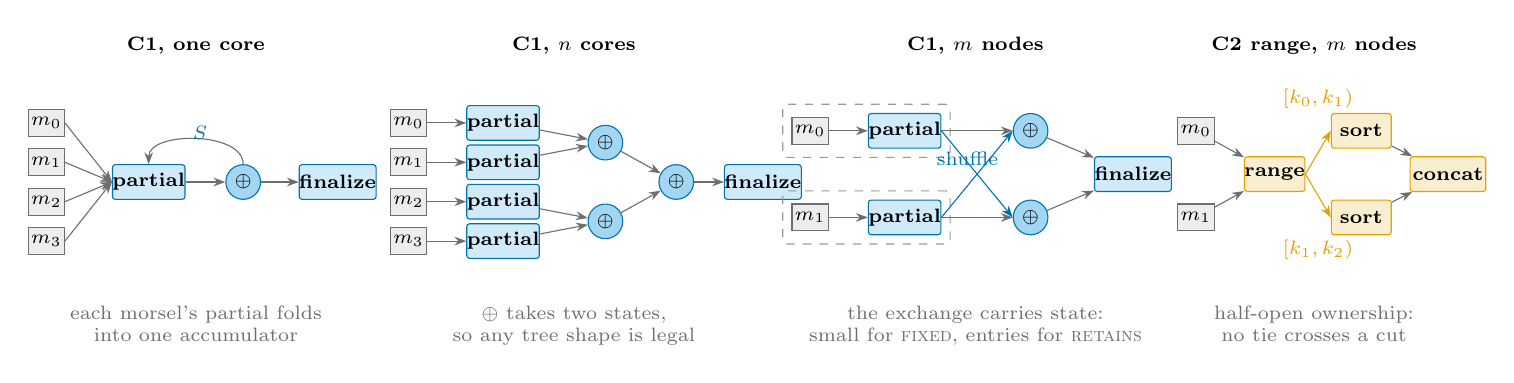
\begin{tikzpicture}[x=1mm, y=1mm,
  bat/.style={draw=pfigGray, fill=pfigLight, minimum width=4.6mm, minimum height=3.4mm,
              inner sep=0pt, font=\scriptsize},
  ph/.style={draw=okBlue, fill=okSky!28, minimum width=8.6mm, minimum height=4.4mm,
             inner sep=0pt, font=\scriptsize\bfseries, rounded corners=1pt},
  cb/.style={draw=okBlue, fill=okSky!55, circle, minimum size=4.4mm, inner sep=0pt,
             font=\scriptsize\bfseries},
  fin/.style={draw=okBlue, fill=okSky!28, minimum width=9.6mm, minimum height=4.4mm,
              inner sep=0pt, font=\scriptsize\bfseries, rounded corners=1pt},
  rng/.style={draw=okOrange, fill=okOrange!18, minimum width=7.6mm, minimum height=4.4mm,
              inner sep=0pt, font=\scriptsize\bfseries, rounded corners=1pt},
  lane/.style={draw=pfigGray!70, dashed, rounded corners=1.5pt, inner sep=1.1mm},
  fl/.style={-{Stealth[length=1.5mm,width=1.1mm]}, draw=pfigGray, line width=0.4pt}]

\begin{scope}
  \node[font=\scriptsize\bfseries, anchor=south] at (19,25.5) {\Ca{}, one core};
  \node[font=\scriptsize, text=pfigGray, anchor=north, align=center] at (19,-4.0)
       {each morsel's partial folds\\into one accumulator};
  \foreach \i in {0,1,2,3}{\node[bat] (a\i) at (0,18-\i*5) {$m_\i$};}
  \node[ph] (ap) at (13,10.5) {partial};
  \node[cb] (ac) at (25,10.5) {$\oplus$};
  \node[fin] (af) at (37,10.5) {finalize};
  \foreach \i in {0,1,2,3}{\draw[fl] (a\i.east) -- (ap.west);}
  \draw[fl] (ap) -- (ac); \draw[fl] (ac) -- (af);
  \draw[fl] (ac.north) .. controls +(0,4.2) and +(0,4.2) .. (ap.north);
  \node[font=\scriptsize, text=okBlue] at (19.5,16.8) {$S$};
\end{scope}

\begin{scope}[xshift=46mm]
  \node[font=\scriptsize\bfseries, anchor=south] at (21,25.5) {\Ca{}, $n$ cores};
  \node[font=\scriptsize, text=pfigGray, anchor=north, align=center] at (21,-4.0)
       {$\oplus$ takes two states,\\so any tree shape is legal};
  \foreach \i in {0,1,2,3}{
    \node[bat] (b\i) at (0,18-\i*5) {$m_\i$};
    \node[ph]  (bp\i) at (12,18-\i*5) {partial};
    \draw[fl] (b\i) -- (bp\i);}
  \node[cb] (bc0) at (25,15.5) {$\oplus$};
  \node[cb] (bc1) at (25,5.5)  {$\oplus$};
  \node[cb] (bc2) at (34,10.5) {$\oplus$};
  \node[fin] (bf) at (45,10.5) {finalize};
  \draw[fl] (bp0) -- (bc0); \draw[fl] (bp1) -- (bc0);
  \draw[fl] (bp2) -- (bc1); \draw[fl] (bp3) -- (bc1);
  \draw[fl] (bc0) -- (bc2); \draw[fl] (bc1) -- (bc2); \draw[fl] (bc2) -- (bf);
\end{scope}

\begin{scope}[xshift=97mm]
  \node[font=\scriptsize\bfseries, anchor=south] at (21,25.5) {\Ca{}, $m$ nodes};
  \node[font=\scriptsize, text=pfigGray, anchor=north, align=center] at (21,-4.0)
       {the exchange carries state:\\small for \textsc{fixed}, entries for \textsc{retains}};
  \foreach \i in {0,1}{
    \node[bat] (c\i) at (0,17-\i*11) {$m_\i$};
    \node[ph]  (cp\i) at (12,17-\i*11) {partial};
    \draw[fl] (c\i) -- (cp\i);
    \node[lane, fit=(c\i)(cp\i)] {};}
  \node[cb] (cc0) at (28,17) {$\oplus$};
  \node[cb] (cc1) at (28,6)  {$\oplus$};
  \node[fin] (cf) at (41,11.5) {finalize};
  \draw[fl] (cp0) -- (cc0); \draw[fl] (cp1) -- (cc1);
  \draw[fl, draw=okBlue] (cp0.east) -- (cc1.west);
  \draw[fl, draw=okBlue] (cp1.east) -- (cc0.west);
  \draw[fl] (cc0) -- (cf); \draw[fl] (cc1) -- (cf);
  \node[font=\scriptsize, text=okBlue, anchor=south] at (20,11.4) {shuffle};
\end{scope}

\begin{scope}[xshift=146mm]
  \node[font=\scriptsize\bfseries, anchor=south] at (15,25.5) {\Cb{} range, $m$ nodes};
  \node[font=\scriptsize, text=pfigGray, anchor=north, align=center] at (15,-4.0)
       {half-open ownership:\\no tie crosses a cut};
  \foreach \i in {0,1}{
    \node[bat] (d\i) at (0,17-\i*11) {$m_\i$};}
  \node[rng] (dr) at (10,11.5) {range};
  \draw[fl] (d0) -- (dr); \draw[fl] (d1) -- (dr);
  \node[rng] (ds0) at (21,17) {sort};
  \node[rng] (ds1) at (21,6)  {sort};
  \draw[fl, draw=okOrange] (dr.east) -- (ds0.west);
  \draw[fl, draw=okOrange] (dr.east) -- (ds1.west);
  \node[fin, draw=okOrange, fill=okOrange!18] (dc) at (32,11.5) {concat};
  \draw[fl] (ds0) -- (dc); \draw[fl] (ds1) -- (dc);
  \node[font=\scriptsize, text=okOrange, anchor=south] at (15.5,18.6) {$[k_0,k_1)$};
  \node[font=\scriptsize, text=okOrange, anchor=north] at (15.5,4.4) {$[k_1,k_2)$};
\end{scope}
\end{tikzpicture}
\caption{How the partitionable contracts map onto schedulers. Under \Ca{} only the arrangement
of $\mathsf{partial}$, $\oplus$ and $\mathsf{finalize}$ changes: one core folds every partial
into one accumulator, $n$ cores combine up a tree, and $m$ nodes exchange state. Associativity
permits any tree shape, commutativity any arrival order. The state class sets what the
exchange carries: 100 accumulators per worker for a 100-group \texttt{SUM}, the input itself
for a \texttt{DISTINCT} over a unique column. The fourth panel shows the range form of \Cb{}:
range-partition, sort, concatenate, with rank offsets computed from per-range counts.}
\label{fig:schedulers}
\end{figure*}

\subsection{The equivalence relation between modes}
\label{sec:equivalence}

``The same result on one core and a hundred nodes'' needs a definition. Under any partition
count and any execution mode (sequential, morsel-parallel, distributed, micro-batch), \sys{}
promises a result \emph{equivalent} to the single-node one. Column names and types are equal,
and so are the row multisets, except in four cases where SQL itself leaves the answer open.
\begin{enumerate}\itemsep0pt \parskip0pt \topsep1pt
\item \emph{Floating-point aggregates} agree up to reassociation. IEEE addition is not
associative, and partition count, morsel boundaries and micro-batch boundaries all change the
summation tree, so batch and micro-batch runs over the same input are not bit-identical either.
\item \emph{An unordered \texttt{LIMIT} $n$} returns exactly $n$ rows, each a row of the
unlimited result, but which $n$ is unspecified. On rows $\{a,b\}$, \texttt{LIMIT 1} may return
either. With an \texttt{ORDER BY} the answer is defined and both paths compute it.
\item \emph{Ties in \texttt{row\_number} and in a distributed sort}: the partitions, their
sizes and the set of numbers are equal, but which tied row receives which number is not.
Peers share a value under \texttt{rank} and \texttt{dense\_rank}, so neither is affected.
\item \emph{An unordered \texttt{array\_agg}} returns the same elements as a multiset, in an
unspecified order; \texttt{array\_agg(order\_by=...)} is deterministic.
\end{enumerate}
The oracle tests check exactly this relation: an order-insensitive multiset comparison with a
float tolerance for unordered results, an ordered comparison wherever the query orders, a
subset-and-count check for unordered \texttt{LIMIT}, and a rank-set check for tied
\texttt{row\_number}.

The relation covers errors in one case. Integer \texttt{SUM} accumulates in \texttt{i64} and
carries its \emph{partial} state as a 128-bit integer, checking only the \emph{final} total
against the \texttt{Int64} result type. A partition whose own total overflows 64 bits thus no
longer errors when the grand total fits: $M + 1 + (-1)$ for the largest representable $M$
gives $M$ under every grouping. Decimal \texttt{SUM} over \texttt{DECIMAL}$(p,s)$ returns
\texttt{DECIMAL}$(38,s)$, as DuckDB does, and raises only past 38 digits. Decimal
\texttt{AVG} and the moments run in \texttt{float64}. Which of two data errors a query reports
first is unspecified, but predicate reordering cannot introduce one. The executor reorders only
conjuncts it can prove infallible, so a filter that shields a strict cast keeps shielding it.

Reassociation also composes, which a tolerance on the final column misses. A last-bit
difference can cross a \texttt{HAVING} threshold or become a different integer through
\texttt{rank()}. TPC-DS q67 ranks a \texttt{SUM} over a \texttt{ROLLUP}: cast to
\texttt{float64}, a last-bit disagreement produced different ranks, while on the source
\texttt{DECIMAL} types all 100 rows match exactly and in order. Floating-point variance,
covariance and the higher moments use Chan's pairwise merge with Neumaier compensation, which
reduces cancellation error without bounding it away. Plain floating \texttt{SUM} and
\texttt{AVG} skip compensation for speed. Bitwise-reproducible summation under a free partition
count is available, at a cost \sys{} has not paid~\cite{demmel2013reproducible}.

\subsection{What the contracts bound, and what they do not}
\label{sec:memory}

The executor streams every query, batch included. Operators pull morsels through pipelines
and materialize only at pipeline breakers~\cite{leis2014morsel}. The memory \carbo{} governs
on one node is
\begin{equation}
M_{\text{node}} \;\le\; \sum_{b \in \text{breakers}} R_b \;+\; \sum_{q \in Q_{\text{node}}} B_q
\;+\; M_{\text{store}},
\label{eq:mem}
\end{equation}
where $R_b$ is breaker $b$'s \emph{resident} state, $B_q$ the bytes in flight on transport
queue $q$, and $M_{\text{store}}$ the published shuffle output a worker holds for its peers.
Each term has its own control. The memory envelope bounds $R_b$: past it, aggregation,
distinct, sort, join build and partitioned windows spill, so a \textsc{retains} operator's
\emph{logical} state (\cref{eq:bound}) can exceed memory while its resident state does not.
$M_{\text{store}}$ is capped at a quarter of RAM and spills beyond it. Credits bound $B_q$. A
producer charges $\lceil \mathit{bytes}/\beta \rceil$ credits for an encoded batch, where
$\beta$ is the 1\,MiB morsel byte cap, so a one-row morsel holding a 100\,MiB tensor consumes
most of the window instead of one slot. Capping the charge just below the window (9 of the
default 16 credits) lets an oversized batch always be admitted, and gives
$B_q \le c\,\beta + r_{\max}$ for a window of $c$ credits, with $r_{\max}$ the largest single
batch. Until this work, a gRPC message ceiling of 4\,MiB made any larger batch unfetchable. The
ceiling is now 2\,GiB, and the credit window, not the ceiling, bounds memory. A per-gather
byte budget (768\,MiB, divided among its streams) times the number of concurrent gathers
bounds receive-side buffering separately.

\Cref{eq:mem} bounds executor-managed memory, not process RSS. Reader decode buffers, Arrow
buffers kept alive by a slice, Python objects and a model framework's allocations fall outside
it; \carbo{} watches process RSS as a pressure signal but reserves nothing for them. Device
memory has a separate pool, outside the envelope, that tracks model weights and KV caches. Nor
is the number of transport queues constant. A gather opens $\max(48, \text{peers})$ streams,
so past 48 peers the per-node queue term grows with the cluster, and only the gather budget
stays fixed per node. Reader batch size once proved the point. Parquet read batches were sized
in rows with no byte term, so 65{,}536 rows of decoded images became a 9.6\,GB allocation that
no downstream credit could see. The reader now targets 16\,MiB per decoded batch.

A Rust test with a counting allocator measures the buffering term directly. It runs the
TPC-H q3/q4/q5 join shape with the build side fixed and the probe side growing, and records
peak additional heap with inputs excluded: about 1\,MB at one and at four million probe rows,
where the materializing executor it replaced grew from 221 to 854\,MB. That holds only where
operators preserve or reduce rows. A high-fan-out join once produced one output batch per
input morsel however large, and a skewed equi-join reached 13.1\,GB RSS. Morselizing the join's
output and slicing its probe input brought the same query to 728\,MB with identical results.
Forty-six passing oracle tests missed that defect, because a correctness suite cannot see a
memory property.

\subsection{The incremental form is the same state transition}
\label{sec:streaming}

A \Ca{} operator that folds each batch through $\mathsf{partial}$ and $\oplus$ never reads its
whole input, as a continuous query requires. Batch and micro-batch operators run the same
kernels and differ only in whether $\mathsf{finalize}$ runs once or per trigger. That claim
concerns kernels alone. A continuous query also needs output-update semantics, progress
tracking, late-data handling and coordinated recovery, which \sys{} has only in the
micro-batch form described here; \cref{sec:limitations} compares it with Flink.

\paragraph{The commit protocol.} Each trigger has a stable \texttt{batch\_id}. The driver
pulls and executes the batch without publishing anything, then records the source offsets for
that \texttt{batch\_id} in a write-ahead log. It writes the sink, then operator state, and
marks the batch committed last. A crash before the commit replays the batch under the same
\texttt{batch\_id}, so correctness on replay falls to the sink. Delta commits carry a
transaction marker $(\mathit{app},\mathit{batch\_id})$ checked before and after the write. Iceberg appends carry
the same pair in the snapshot summary, and a table property also keeps the latest committed
version so snapshot expiry does not erase it. A file sink names its output by batch. A keyed
database sink upserts. Each of these makes a replayed batch a no-op. An unkeyed append to a
plain database table does not, and is documented as at-least-once. When the micro-batch itself
runs distributed, only the Delta publish carries the transaction check today, so \sys{}
refuses a distributed streaming write to Iceberg rather than silently downgrading it.

\paragraph{Checkpoint cost.} Recording the \emph{partial} a trigger folded in is sound,
because by \cref{eq:merge} a base state plus every later partial is the state. A delta need
not beat a snapshot: a stream touching every group each trigger produces a delta the size of
the state. \sys{} writes a delta only when it is at most half the state and the deltas since the
last base, this one included, sum to at most the size of the current state $S$. Otherwise it writes a new base and resets the
sum. A configured length also caps the chain. Between two bases at most $2S$ bytes are written
(a base plus deltas summing to at most $S$), against one full snapshot per trigger for the
snapshot-only scheme, and a restore reads one base and at most the configured number of
deltas. A test pins the adversarial case: constant state, with half the groups updated on each
of ten triggers.

\paragraph{Eviction and late data.} A delta chain must also express removal, or replay would
resurrect a closed window. The unwatermarked aggregate never evicts. The windowed aggregate
removes a prefix of a totally ordered event-time axis, so each delta records the eviction bound
it was taken under, and a restore re-applies the largest one after combining. The watermark is
the minimum over active partitions of their maximum event time. An idleness timeout (60\,s by
default) keeps a silent partition from holding it back. A record arriving below the watermark,
even from a partition that resumes after timing out, is dropped and counted; windows already
emitted do not change. There is no side output.

% ===========================================================================
\section{Programming model}
\label{sec:interface}
% ===========================================================================

\begin{figure}[tbp]
\begin{lstlisting}
import batcher as bt

# `path` and `width` come from the reader, not from
# the pixels: the glob yields one row per file with
# its URI and JPEG header fields already populated.
frames = (bt.read.images("s3://clips/**/*.jpg")
     .with_columns(sku=bt.col("path")
                      .str.extract(r"/sku=([^/]+)/")))
cat = bt.read.parquet("s3://catalog/")

hot = (frames
    .filter(bt.col("width") >= 640)    # header, not pixels
    .with_columns(t=bt.col("image")
                    .image.to_tensor(224, 224))
    .ml.infer("resnet50", column="t",
              output_column="label")   # a GPU operator
    .join(cat, on="sku")               # C2: hash exchange
    .group_by("label")                 # C1: merge
    .agg(n=bt.col("sku").count()))

hot.collect(distributed="auto")        # the scale knob
\end{lstlisting}
\caption{A \sys{} program. Decode and inference share one logical plan with the join and the
aggregation. The reader fills the JPEG header field \texttt{width} without decoding, so the
optimizer can sink the filter below \texttt{image.to\_tensor}. A filter on decoded pixels would
have to stay put. Only the model framework's own forward pass runs Python over data here, on
whole batches. Scale appears once, on the last line.}
\label{fig:program}
\end{figure}

SQL is restrictive and so optimizable; a user-defined function is expressive and so opaque.
\sys{} answers this old bargain three ways, in order of preference. The first removes the
callback. \texttt{col("x") * col("y")}, \texttt{.str.contains(...)},
\texttt{.image.to\_tensor(...)} and \texttt{.audio.mel\_spectrogram(...)} all lower to the same
\texttt{bc\_expr::Expr} the SQL front end produces, so each is optimized and executed in Rust,
and the JIT may compile it. This lets the filter in \cref{fig:program} sink below the decode.
Where a callback is needed, \sys{} makes it batch-first. A UDF takes and returns a whole Arrow
\texttt{RecordBatch}, and a class-based UDF keeps a loaded model across batches, which warm GPU
pools depend on. SQL stays, and parses to the same \texttt{LogicalPlan}.

``Python never touches a row'' therefore holds on the relational and expression path only. A
user callback is Python by construction and a model framework runs its own code; \sys{} keeps
both batch-sized. A \texttt{Dataset} is lazy and immutable (each operation returns a new one),
and nothing runs before a terminal call, so the program cannot know how many machines will run
it. \texttt{distributed="auto"} decides at that call. It declines a cluster for an
80{,}000-row filter whose dispatch would cost more than the query, and takes the staged
distributed path for any plan whose shape needs it.

% ===========================================================================
\section{Models as operators}
\label{sec:pipeline}
% ===========================================================================

\begin{figure}[tbp]
\centering
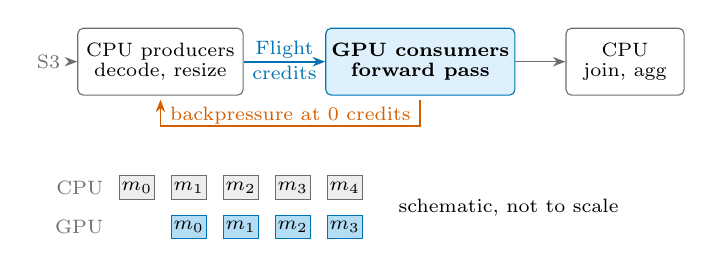
\begin{tikzpicture}[x=1mm,y=1mm,
  pool/.style={draw=pfigGray, fill=white, rounded corners=2pt, inner sep=2pt,
               font=\scriptsize, align=center, minimum height=8.5mm},
  dev/.style={pool, draw=okBlue, fill=okSky!20, font=\scriptsize\bfseries},
  mor/.style={draw=pfigGray, fill=pfigLight, minimum width=4.4mm, minimum height=3.0mm,
              inner sep=0pt, font=\scriptsize},
  fl/.style={-{Stealth[length=1.6mm,width=1.2mm]}, draw=pfigGray, line width=0.5pt}]

  \node[pool, minimum width=21mm] (cpu) at (0,10)  {CPU producers\\[-1pt]{\scriptsize decode, resize}};
  \node[dev,  minimum width=21mm] (gpu) at (33,10) {GPU consumers\\[-1pt]{\scriptsize forward pass}};
  \node[pool, minimum width=15mm] (agg) at (59,10) {CPU\\[-1pt]{\scriptsize join, agg}};
  \node[font=\scriptsize, text=pfigGray, anchor=east] at (-11.5,10) {S3};
  \draw[fl] (-11,10) -- (cpu.west);
  \draw[fl, draw=okBlue, line width=0.8pt] (cpu) --
        node[font=\scriptsize, above, text=okBlue, inner sep=1pt]{Flight}
        node[font=\scriptsize, below, text=okBlue, inner sep=1pt]{credits} (gpu);
  \draw[fl] (gpu) -- (agg);
  \draw[{Stealth[length=1.6mm]}-, draw=okVermillion, line width=0.7pt]
        ($(cpu.south)+(0,-0.5)$) -- ++(0,-3.4) -| ($(gpu.south)+(0,-0.5)$);
  \node[font=\scriptsize, text=okVermillion] at (16.5,3.2) {backpressure at 0 credits};

  \node[font=\scriptsize, text=pfigGray, anchor=east] at (-6,-6)  {CPU};
  \node[font=\scriptsize, text=pfigGray, anchor=east] at (-6,-11) {GPU};
  \foreach \i in {0,1,2,3,4}{
    \node[mor, fill=pfigLight] at (-3+\i*6.6,-6) {$m_{\i}$};}
  \foreach \i in {0,1,2,3}{
    \node[mor, draw=okBlue, fill=okSky!45] at (3.6+\i*6.6,-11) {$m_{\i}$};}
  \node[font=\scriptsize, text=black, anchor=west, align=left] at (29,-8.5)
       {schematic, not to scale};
\end{tikzpicture}
\caption{One plan, two resource pools. CPU producers decode and preprocess while GPU consumers
run the model. Batches cross between them on the shuffle's credit-bounded Flight
transport~\cite{arrowflight}, so a slow consumer applies backpressure. The timeline sketches
the intended overlap (decode of $m_{k+1}$ during the forward pass of $m_k$) and is not a trace
(\cref{sec:eval-gpu} measures the effect). \sys{} splits at one resource boundary per plan, so
the third stage of a CPU$\rightarrow$GPU$\rightarrow$CPU chain runs in the consumer pool.}
\label{fig:gpu}
\end{figure}

For a model in a pipeline, visibility beats feature count: \sys{} makes decode and inference
expressions, which the optimizer sees alongside the relational operators around them. Image decode, crop, resize and tensor normalization run as Arrow kernels
in the data plane, as do audio decode and resampling along with the mel-spectrogram and MFCC
transforms. Vector distances and embedding pooling are expressions too. Over the same corpus
\sys{} decodes $6.4$ to $6.6\times$ faster than Ray Data's \texttt{read\_images}. The paths also
differ in decoder library, thread count and resize semantics, which the experiment does not
separate out.

\paragraph{The inference contract.} A model call carries obligations a relational operator
does not. An expression that references a model binds the model's weights into its identity,
along with the tokenizer and preprocessing, so a new checkpoint is a new expression and never a
silently changed answer. Precision is bound in too. By default \sys{} runs inference under FP16
autocast on devices that support it, a numerical choice any comparison must match or disclose.
Batch size is \emph{not} fixed. The engine derives a default
from row width and the device's free memory, splits the tail, and halves any batch that raises
a CUDA out-of-memory error. That is legal only for models whose per-row output ignores the
other rows in the batch. Models run in evaluation mode under \texttt{inference\_mode}, which
removes the dropout and batch-statistics cases. A padded sequence model must mask its own
padding; the engine does not check that it does. The residual batch dependence is numerical: another batch size can select
other kernels and move low-order bits under FP16. \sys{} therefore promises agreement of
predictions across batch sizes (labels, argmax, generated tokens under greedy decoding) rather
than bit-equal logits. Stochastic generation falls outside the contract.

\paragraph{One scheduler across CPU and GPU.}
\label{sec:gpu}
Run a chain of unlike costs inside one worker and the accelerator idles through every decode.
Users usually hand-tune a per-stage CPU-to-GPU worker ratio. In \sys{} the engine owns that
scheduling problem (\cref{fig:gpu}). Each pool runs its sub-plan through the ordinary
executor, so the split moves placement and leaves semantics alone. Ray Data's streaming batch
model~\cite{luan2025streamingbatch} attacks the same problem. Its unit of execution is the
partition, which buys elasticity and partition-level fault tolerance that \sys{} lacks. \sys{}
instead keeps both stages in one plan, under one cost model with the joins around them.

% ===========================================================================
\section{Measurement-driven optimization}
\label{sec:learning}
% ===========================================================================

\begin{figure}[tbp]
\centering
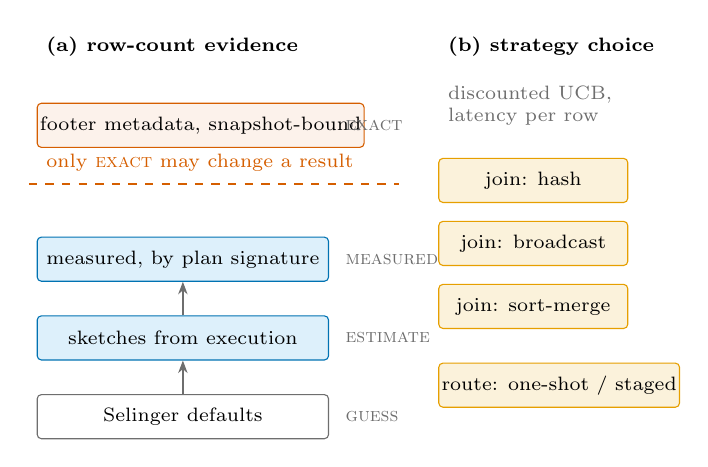
\begin{tikzpicture}[x=1mm,y=1mm,
  rung/.style={draw=pfigGray, fill=white, minimum width=37mm, minimum height=5.6mm,
               inner sep=1pt, font=\scriptsize, rounded corners=1.5pt, anchor=west},
  rungN/.style={rung, draw=okBlue, fill=okSky!20},
  arm/.style={draw=okOrange, fill=okOrange!14, minimum width=24mm, minimum height=5.6mm,
              inner sep=1pt, font=\scriptsize, rounded corners=1.5pt, anchor=west},
  prov/.style={font=\scriptsize, text=pfigGray, anchor=west},
  up/.style={-{Stealth[length=1.6mm,width=1.2mm]}, draw=pfigGray, line width=0.5pt}]
  \node[font=\scriptsize\bfseries, anchor=west] at (0,47) {(a) row-count evidence};
  \node[rung]  (a) at (0,0)    {Selinger defaults};
  \node[rungN] (c) at (0,10)   {sketches from execution};
  \node[rungN] (d) at (0,20)   {measured, by plan signature};
  \node[rung, draw=okVermillion, fill=okVermillion!8] (b) at (0,37) {footer metadata, snapshot-bound};
  \foreach \x/\y in {a/c,c/d}{\draw[up] (\x.north) -- (\y.south);}
  \node[prov] at (38,0)  {\textsc{guess}};
  \node[prov] at (38,10) {\textsc{estimate}};
  \node[prov] at (38,20) {\textsc{measured}};
  \node[prov] at (38,37) {\textsc{exact}};
  \draw[draw=okVermillion, line width=0.8pt, dashed] (-1,29.5) -- (46,29.5);
  \node[font=\scriptsize, text=okVermillion, align=left, anchor=west] at (0,32.2)
       {only \textsc{exact} may change a result};
  \node[font=\scriptsize\bfseries, anchor=west] at (51,47) {(b) strategy choice};
  \node[arm] (h) at (51,30) {join: hash};
  \node[arm] (bc) at (51,22) {join: broadcast};
  \node[arm] (sm) at (51,14) {join: sort-merge};
  \node[arm] (rt) at (51,4) {route: one-shot / staged};
  \node[font=\scriptsize, text=pfigGray, align=left, anchor=west] at (51,39.5)
       {discounted UCB,\\latency per row};
\end{tikzpicture}
\caption{\kyber{} makes two kinds of learned decision. (a) Row-count evidence, by precedence
for estimates: a measured count for the same plan signature beats a sketch, and a sketch beats
a default. None of these may change a result. Two rewrites can, dropping a \texttt{DISTINCT}
over a provably unique key and replacing a provably empty subtree, and they read only exact
footer evidence bound to the snapshot of the source they rewrite. (b) Strategy choice, kept
apart from estimation. A bandit~\cite{auer2002ucb} picks among result-equivalent join
algorithms and between one-shot and staged distributed execution.}
\label{fig:kyber}
\end{figure}

An engine that cannot price its data before running must invent the numbers, as a static cost
model does, or measure itself and plan from what it saw. \sys{} measures (\cref{fig:kyber}), and one rule keeps
that safe: every learned value selects among result-equivalent alternatives. Each
bandit arm computes the same relation. A threshold chooses between algorithms that compute the
same function, and a partition count only shards. Learning can move how much memory a query
reserves, when it spills, how wide a batch is and which equivalent algorithm runs. It cannot
move the answer, and a test holds that a cold store reproduces the untuned engine's results.
Learned optimizers that predict plans~\cite{marcus2019neo,marcus2021bao,kipf2019learned} are
not unsafe either, since a validated optimizer steered by hints keeps its semantics. \sys{}
bounds a bad model's damage by construction instead, at the price of a weaker signal.

\paragraph{Stores and their keys.} Three stores feed planning. \emph{Row counts} are filed
under the plan signature of the operator they measure, a hash over the plan's structure with
literals normalized, to which a scan contributes its source identity. For a lakehouse table
that identity includes the snapshot or version. For plain files, the learned count carries the
files' size-and-modification digest and is ignored once the digest stops matching. When a
query's root is a projection over an aggregate, its count goes under the aggregate, the node
the estimator corrects. Counts update by an exponentially weighted mean and enter estimates as
a clipped, shrunk correction to the model's own estimate. \emph{Cost coefficients} (work units
per row for scan, filter, hash build and probe, sort and the rest) are refit from per-operator
timings every 64 new observations, shrunk toward their defaults with weight $n/(n+20)$ and
clamped within $10\times$ of them. The model's objective weights CPU work, I/O bytes and
network bytes, counting network double. A hardware fingerprint (CPU model and count, SIMD
width, cache sizes, memory size class, disk class, GPU) keys the coefficients and bandit state,
so a measurement from one machine never prices a plan on another. Row counts skip it, being
independent of the machine. \emph{Strategy statistics} feed a
bandit over two decisions: the join algorithm per join signature (hash, broadcast, sort-merge)
and the distributed route per plan (one-shot or staged). The bandit minimizes latency per
million input rows with a discounted, variance-scaled lower-confidence rule. Until an arm has
three discounted observations it defers to the cost model. Ties break by arm name, and the
first observation of a route arm is dropped as a cold-start outlier.

\paragraph{Three timescales.} Two mechanisms run inside an operator at microsecond grain, each
standing in for a number a static model would invent. A conjunctive filter orders its
infallible predicates by measured time per row removed. On a shape built with two equal-cost
predicates, only one of them selective, that is worth $1.86\times$. A parallel aggregate
samples the first $\max(4, m/16)$ of its $m$ morsels. If grouping reduced them below 20\%, it
folds partials per morsel. Otherwise it pre-partitions by key, the third panel of
\cref{fig:schedulers} run across cores, and gains $3.7\times$ when grouping reduces nothing.
Because the sample is the first morsels, an input with unrepresentative early rows can pick the
slower strategy; both strategies return the same relation. At a pipeline breaker the engine
re-plans the remainder on real cardinalities. Spark AQE~\cite{sparkaqe} works at the same
mechanism and grain, but \sys{} runs it on one node as well as on a cluster. It engages only
on a plan with a join whose stages each clear 5M rows or about 320\,MB, or on any distributed
plan whose shape needs staging. Across executions the engine accumulates the three stores
above, and \cref{sec:eval-learning} measures what they buy.

A measurement buys less than the word suggests. Applying a sampled reduction ratio to
unprocessed morsels is an inference, and so is applying a fitted crossover to an unseen size.
Safety rests on result invariance alone, whatever ``measured'' seems to promise.
% ===========================================================================
\section{Runtime}
\label{sec:arch}
% ===========================================================================

Three structural rules carry the runtime. Each exists because breaking it is silent.
\emph{The subsystems may not import one another.} An optimizer pass that collects its own
telemetry compiles and passes every test while corrupting the loop \cref{sec:learning}
depends on. A lint contract blocks that category of coupling, though not every instance.
\emph{One expression type serves every CPU tier}, and the crate graph points one way, so no
new backend can introduce a second definition of what a plan node means
(\cref{sec:arch-overview} gives the JIT and cuDF checks). Device values are checked only by an
opt-in shadow run on the CPU engine, which needs real hardware.

\paragraph{\carbo{}, the resource manager.} \carbo{} decides whether a plan fits and when a
query goes out of core, reserves memory, and hands out shuffle credits. It neither rewrites
nor computes (\cref{fig:carbonite}). A yes-or-no admission answer gives a planner nothing
smaller to try, so \carbo{}'s verdict names the binding constraint, the operator that binds and
suggested bounds. Computed once per query, it does not loop. A memory-infeasible plan with a
spill path goes to the spilling executor, its partition count floored at the suggested bound.
Otherwise an infeasible plan raises a \texttt{PlanError} naming the operator. Flow control uses
credits (\cref{sec:memory}). Tearing down a consumer's stream releases a producer blocked on
its credits. A consumer that hears nothing for 60 seconds abandons the fetch and enters the
recovery path below.

\begin{figure}[tbp]
\centering
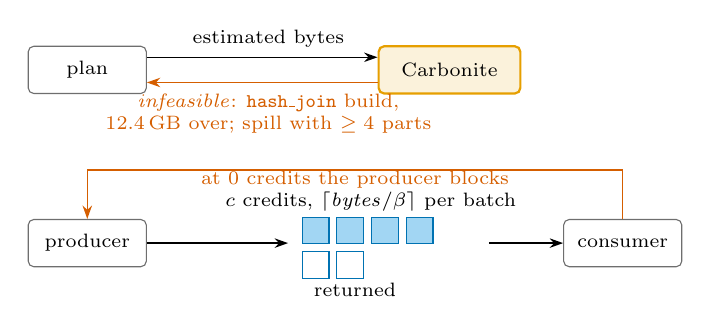
\begin{tikzpicture}[x=1mm,y=1mm,
  b/.style={draw=pfigGray, fill=white, rounded corners=2pt, inner sep=2pt,
            font=\scriptsize, align=center, minimum height=6mm},
  o/.style={b, draw=okOrange, fill=okOrange!14, line width=0.8pt},
  slot/.style={draw=okBlue, minimum width=3.4mm, minimum height=3.4mm, inner sep=0pt},
  a/.style={-{Stealth[length=1.7mm,width=1.2mm]}, draw=black, line width=0.55pt},
  lb/.style={font=\scriptsize, inner sep=1pt}]
  \node[b, minimum width=15mm] (k) at (0,0)  {plan};
  \node[o, minimum width=18mm] (c) at (46,0) {\carbo{}};
  \draw[a] ($(k.east)+(0,1.6)$) -- ($(c.west)+(0,1.6)$);
  \node[lb, anchor=south] at (23,2.4) {estimated bytes};
  \draw[a, draw=okVermillion] ($(c.west)+(0,-1.6)$) -- ($(k.east)+(0,-1.6)$);
  \node[lb, text=okVermillion, anchor=north, align=center] at (23,-2.6)
       {\emph{infeasible}: \texttt{hash\_join} build,\\12.4\,GB over; spill with $\ge 4$ parts};
  \node[b, minimum width=15mm] (p) at (0,-22)  {producer};
  \node[b, minimum width=15mm] (r) at (68,-22) {consumer};
  \foreach \i in {0,1,2,3}{\node[slot, fill=okSky!55] at (29+\i*4.4,-20.4) {};}
  \foreach \i in {0,1}{\node[slot, fill=white] at (29+\i*4.4,-24.8) {};}
  \node[lb, anchor=south] at (36,-18.4) {$c$ credits, $\lceil\mathit{bytes}/\beta\rceil$ per batch};
  \node[lb, anchor=north] at (34,-26.6) {returned};
  \draw[a] (p.east) -- (25.5,-22);
  \draw[a] (51,-22) -- (r.west);
  \draw[a, draw=okVermillion] (r.north) -- ++(0,6.2) -| (p.north);
  \node[lb, text=okVermillion, anchor=south] at (34,-15.4) {at 0 credits the producer blocks};
\end{tikzpicture}
\caption{\carbo{}'s two interfaces. Above, admission returns the binding constraint and the
operator that binds, and its suggested bound sets the spill partition count. Below,
credit-based flow control charges by bytes in units of the morsel cap $\beta$, so one
oversized row cannot slip past the window as a single slot.}
\label{fig:carbonite}
\end{figure}

\paragraph{Core, the executor.} Core runs the plan it is given and reports what happened. It
rewrites no plan, though it makes two operator-local choices between result-equivalent
strategies. A conjunctive filter orders its infallible predicates by measured cost per row
removed. A parallel aggregate keeps a hash table per morsel or pre-partitions by key, depending
on the reduction a sample of morsels achieved. Each operator records its chosen strategy beside
its row counts and timings, so every Metadata Hub entry carries the decision it was taken under
(\cref{fig:core}).

\begin{figure}[tbp]
\centering
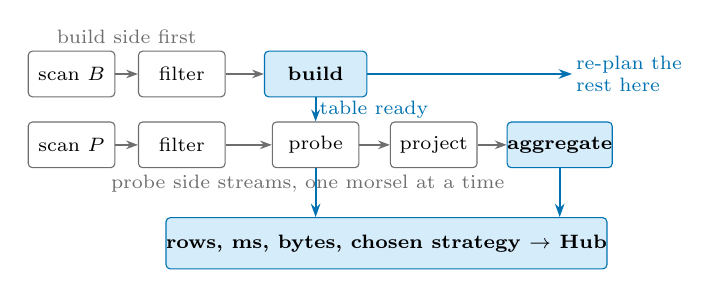
\begin{tikzpicture}[x=1mm,y=1mm,
  op/.style={draw=pfigGray, fill=white, minimum width=11mm, minimum height=5.8mm,
             inner sep=0pt, font=\scriptsize, rounded corners=1.5pt},
  brk/.style={op, draw=okBlue, fill=okSky!25, font=\scriptsize\bfseries, minimum width=13mm},
  a/.style={-{Stealth[length=1.5mm,width=1.1mm]}, draw=pfigGray, line width=0.5pt},
  lb/.style={font=\scriptsize, inner sep=1pt}]
  \node[op]  (sc2) at (0,9)  {scan $B$};
  \node[op]  (fi2) at (14,9) {filter};
  \node[brk] (bu)  at (31,9) {build};
  \node[op]  (sc)  at (0,0)  {scan $P$};
  \node[op]  (fi)  at (14,0) {filter};
  \node[op]  (pb)  at (31,0) {probe};
  \node[op]  (pr)  at (46,0) {project};
  \node[brk] (ag)  at (62,0) {aggregate};
  \draw[a] (sc2) -- (fi2); \draw[a] (fi2) -- (bu);
  \draw[a] (sc) -- (fi); \draw[a] (fi) -- (pb); \draw[a] (pb) -- (pr); \draw[a] (pr) -- (ag);
  \draw[a, draw=okBlue, line width=0.8pt] (bu) -- node[lb, right, text=okBlue]{table ready} (pb);
  \node[lb, text=pfigGray, anchor=south] at (7,12.4) {build side first};
  \node[lb, text=pfigGray, anchor=north] at (30,-3.4) {probe side streams, one morsel at a time};
  \draw[-{Stealth[length=1.7mm,width=1.2mm]}, draw=okBlue, line width=0.9pt]
       (bu.east) -- ++(26,0) node[lb, right, text=okBlue, align=left]{re-plan the\\rest here};
  \node[brk, minimum width=44mm, minimum height=6.5mm] (hub) at (40,-12.5)
       {rows, ms, bytes, chosen strategy $\rightarrow$ Hub};
  \draw[-{Stealth[length=1.7mm,width=1.2mm]}, draw=okBlue, line width=0.8pt] (ag.south) -- (ag.south |- hub.north);
  \draw[-{Stealth[length=1.7mm,width=1.2mm]}, draw=okBlue, line width=0.8pt] (pb.south) -- (pb.south |- hub.north);
\end{tikzpicture}
\caption{Core's execution model for a join feeding an aggregate. The build input runs to
completion before the probe input streams through the probe, the projection and the aggregate,
one morsel at a time. The finished build gives the engine its first exact cardinality, and the
stage-boundary re-plan happens there. Every operator reports rows, time, bytes and its chosen
strategy to the Metadata Hub.}
\label{fig:core}
\end{figure}

\subsection{Recovery is a protocol, not a corollary of the algebra}
\label{sec:recovery}

Associativity and commutativity let valid partials be reordered. They say nothing about
duplicating or dropping one, and \texttt{SUM} and \texttt{COUNT} are not idempotent, so worker
loss and retry need a protocol above the algebra. \sys{}'s has four parts.

\emph{Identity.} A published bucket is named by
$(\mathit{query}, \mathit{stage}, \mathit{source}, \mathit{destination}, \mathit{epoch})$,
where the query identifier is a random 63-bit value per query and the source is the map
partition's index within the stage. For the aggregate reduce, the driver allocates epochs per
source. A recompute republishes at the next epoch and reducers fetch exactly the epoch the
driver names, so a late publication from an abandoned attempt sits in the store unread. The
join, sort and window shuffles reach the same effect differently: they retire a lost source's
replicas, then relocate it to a new worker address.

\emph{Completeness.} Every map publication in the aggregate, join, sort, window and global
window shuffles returns the row count of each bucket it wrote, and the driver passes the counts
to the reducers along with the addresses. On every delivery path a reducer compares, per
source, what it received with what was published. A shortfall (a missing ticket, a truncated
stream, a replica copied from a missing primary) falls over to a replica, then to the recompute
path a dead worker takes. Fetching a ticket the peer does not hold raises a retryable error
rather than yielding an empty bucket. Only a bucket published empty is expected empty. A short
relation therefore fails the stage or gets recomputed, and is never returned. Interior levels
of the combiner tree fail closed on a missing partial but carry no counts.

\emph{Publication.} Replication copies each published bucket to a survivor. It acknowledges
only once every ticket in the set is republished with its count verified, and the driver
advertises replicas only after every stage has acknowledged. Recovery retires a source's
replicas before republishing it.

\emph{Interior of the combiner tree.} A tree-reduce builds its interior fallbacks inside one
call. If an interior node fails, the attempt raises, a ping finds the dead workers, lost leaves
are recomputed and the whole tree is rebuilt. Interior outputs are named by tree position and
map to the same logical chunk across attempts, so a zombie's late publication carries the same
rows as the replacement's. The tree does not yet count-check a partial the zombie only
half-wrote. It relies on the publish being atomic.

\paragraph{Replayability.} Recomputing a lost split assumes a source immutable for the query
and deterministic operators. File sources are read at the snapshot the plan bound, lakehouse
tables at a snapshot identifier. User callbacks are assumed pure. One with external side
effects can run twice under recovery, and \sys{} does not detect it.

% ===========================================================================
\section{Evaluation}
\label{sec:eval}
% ===========================================================================

\Cref{tab:protocol} gives each experiment tag's hardware, date, lineup, repetition and
statistic. No timing is reported for a query whose result disagrees with DuckDB under
\cref{sec:equivalence} (floats within $1.5\times10^{-6}$ absolute, $10^{-9}$ relative). Model
workloads are gated on prediction agreement. Every engine is measured up to a materialized \texttt{pyarrow.Table}.

\begin{table*}[tbp]
\centering\scriptsize
\setlength{\tabcolsep}{3pt}
\begin{tabular}{@{}l>{\raggedright\arraybackslash}p{0.22\textwidth}>{\raggedright\arraybackslash}p{0.19\textwidth}l>{\raggedright\arraybackslash}p{0.25\textwidth}l@{}}
\toprule
Tag & Experiment & Hardware & Date & Lineup, isolation, repetition & Statistic \\
\midrule
\E{1} & six single-node suites (\cref{tab:single}, top) & 48-core (24 + SMT), 92\,GiB, shared & 2026-09-13 & 4 engines, one process per case, 5 runs & min per case; geomean \\
\E{2} & TPC-H sf10, JOB; TPC-DS sf1 (\cref{tab:single}, bottom) & 96-core, 184\,GiB; TPC-DS on \E{1}'s box & 08-25; 09-11 & 2 engines, in-process, 5 runs & min per case; geomean \\
\E{3} & scheduler equivalence (\cref{sec:eval-algebra}) & \E{1}'s box, local Ray & 2026-09-23 & \texttt{distributed=False} vs.\ 2 workers & agree / differ \\
\E{4} & CPU cost, TPC-H sf1 & 96-core, 184\,GiB & 2026-08-18 & 2 engines, in-process, 2 rounds & \texttt{getrusage}; geomean \\
\E{5} & cold small queries & 96-core, load $\approx$18 & 2026-07-29 & fresh literal per run & median of 10 \\
\E{6} & streaming backlog drain & 96-core; batch arm on \E{1}'s box & 08-18; 09-23 & per engine, 5 runs & median \\
\E{7} & TPC-H sf100 pipelines (\cref{tab:cluster}) & 1 head (no worker CPU) $+$ 100$\times$(4 CPU, 8\,GB) & 2026-09-09 & engine-major, best of 2, 400\,s timeout & min \\
\E{8} & worker loss (\cref{tab:faults}) & 8 workers, one box, local Ray & 2026-08-18 & 3 rounds per arm & min \\
\E{9} & image scoring, 100k JPEGs & 6$\times$g4dn.2xlarge (T4) & 2026-09-06 & engine-major, 1 run & wall \\
\E{10} & GPU workloads (\cref{tab:gpu}) & 8$\times$T4 nodes $+$ 8 CPU nodes & Jul.--09-09 & \sys{}; Ray Data where named & wall, NVML \\
\E{11} & learning vs.\ plan-cache ablation (\cref{fig:learning}) & \E{1}'s box, shared & 2026-09-23 & fresh process per arm, 8 runs, 4 rounds & geomean vs.\ own run 8 \\
\E{12} & repeated TPC-H sf1 and H2O \texttt{group\_by} & \E{1}'s box, shared & 2026-09-23 & 4 engines, one process per case, best of 5, 5 repeats & median and range of geomeans \\
\bottomrule
\end{tabular}
\caption{Experiment protocol; every number in the paper carries one of these tags. ``Shared'':
other work ran on the machine. On \E{1}'s box, \texttt{-{}-repeat 5} gave a suite-geomean spread
of 1.4 to 2.3\% (11\% for a single case), so suite ratios a few percent apart do not differ.}
\label{tab:protocol}
\end{table*}

\subsection{Do the schedulers agree?}
\label{sec:eval-algebra}

Beyond the property test of \cref{eq:merge}, an operator matrix crosses every execution mode
(collect, spill, streamed batches, distributed) with every value edge (nulls, empty input, one
row, duplicates, $-0.0$ and NaN, descending order). The defects that reached users were each a
non-default flag on a non-default path that every single-axis test passed: a descending sort
returned unsorted data under spill, and a distributed \texttt{GROUP BY} on a float key split a
group in two.

Alone, \texttt{distributed=True} runs one worker, which computes what one node computes. \E{3}
therefore compares \texttt{distributed=False} with two workers on TPC-H sf1 over Parquet split
eight ways, since an in-memory table cannot be divided and would keep the distributed side on
one worker. A control known to diverge, \texttt{LIMIT 3} over an unordered \texttt{group\_by},
must return three rows of the full aggregate but may pick different ones. It moved: single-node
kept groups $\{3,7,10\}$, two workers $\{3,5,12\}$. Against that, all 22 queries returned
equivalent relations, each on two workers over two partitions.

At four workers the run first failed q10 and q13 with a truncated shuffle file, rewritten in
place by a straggler's backup task while a reducer read it. Shuffle files now go to a private
temporary and are renamed into place, after which 32 repeats of q3, q10, q13 and q18 at four
workers agreed. The earlier version of this experiment ran one worker on unsplittable tables,
which is why it never saw the defect.

\subsection{Single-node relational}
\label{sec:eval-tpch}

\begin{table}[tbp]
\centering\footnotesize
\setlength{\tabcolsep}{2.6pt}
\begin{tabular}{@{}lrrrrr@{}}
\toprule
& & \multicolumn{2}{c}{DuckDB} & & \\
\cmidrule(lr){3-4}
Suite & $n$ & Arrow & native & Polars\cite{polars} & slower \\
\midrule
JSON                                & 5   & \win \textbf{0.32} & \win \textbf{0.35} & \win \textbf{0.01} & \win 0/5 \\
H2O.ai~\cite{h2obenchmark} \texttt{join} & 5   & \win \textbf{0.58} & \win \textbf{0.63} & \win \textbf{0.51} & \win 0/5 \\
ClickBench~\cite{clickbench}$^{*}$  & 43  & \win \textbf{0.16} & \win \textbf{0.65} & \win \textbf{0.37} & 15/43 \\
TPC-H~\cite{tpch} sf1               & 22  & \win \textbf{0.25} & \win \textbf{0.72} & \win \textbf{0.54} & 6/22 \\
Operator mix$^{*}$                  & 46  & \win \textbf{0.47} & \win \textbf{0.75} & \win \textbf{0.16} & 13/46 \\
H2O.ai \texttt{group\_by}           & 10  & \win \textbf{0.83} & 1.05               & \win \textbf{0.53} & 6/10 \\
\midrule
\multicolumn{6}{@{}l@{}}{\emph{\E{2}: larger data and harder planning; separate runs}} \\
TPC-H sf10, in-memory               & 22  & --- & \win \textbf{0.963} & --- & --- \\
TPC-DS~\cite{tpcds} sf1             & 99  & --- & \win \textbf{0.98}  & --- & --- \\
Join Order~\cite{leis2015goodjoin}  & 113 & --- & \loss 1.11          & --- & --- \\
\bottomrule
\end{tabular}
\caption{Single-node relational results, \bx{}; below 1.00 means \sys{} is faster. Top: \E{1},
every case correctness-gated for every engine; the \E{1} logs keep suite ratios but not
per-engine failed-case counts, which \E{12} records. The last column counts cases where any
engine beat \sys{}. Bottom: \E{2}, comparable within a row only. $^{*}$Includes five ClickBench
queries and two operator-mix cases answered from a recorded statistic without executing
(\cref{sec:eval-exec}).}
\label{tab:single}
\end{table}

\Cref{tab:single} has \sys{} leading DuckDB on all six \E{1} suites over identical Arrow, from
$0.83$ on H2O \texttt{group\_by} to $0.16$ on ClickBench. Against the compressed native store it
leads five and ties on H2O \texttt{group\_by} ($1.05$ here, $0.95$ three days later on a loaded
box, both inside the spread of \cref{tab:protocol}). \E{12} repeats two suites five times for
intervals. On TPC-H sf1 \sys{} measured $0.86$ against DuckDB-native (range $0.75$ to $0.88$),
$0.30$ against DuckDB over Arrow and $0.55$ against Polars; on H2O \texttt{group\_by}, $1.03$
against DuckDB-native ($1.00$ to $1.04$), $0.79$ over Arrow and $0.49$ against Polars. Every
engine passed every case in every repeat.

That run qualifies \cref{tab:single} twice. Its native-store TPC-H ratio, $0.86$ against \E{1}'s
$0.72$, shows one sweep on a loaded machine moving by more than the quiet-box spread. And the
geometric mean disagrees with the sum: the median TPC-H suite \emph{sum} was 715\,ms for \sys{}
and 716\,ms for DuckDB-native, a tie, because \sys{} wins most short queries and loses long ones
such as q21 (108 against 72\,ms).

The lower block depends on conditions. TPC-H sf10 at $0.963$ reads in-memory Arrow on the
96-core box. From Parquet files on a loaded 48-core box (2026-09-16) the same suite measured
$1.52$, losing 21 of 22 queries, and that is what a user with files on disk gets. The
single-node crossover with DuckDB thus lies between sf1 and sf10, depending on how data arrives.
TPC-DS completed all 99 queries at $0.98$ with every check passing. A later run on a loaded box
read $0.99$ to $1.40$ across two passes, a spread due to load. \sys{} loses the Join Order
Benchmark, whose correlated predicates defeat independence assumptions~\cite{leis2015goodjoin}:
its total time beats DuckDB's (8.1\,s against 8.9) but its geometric mean is 11\% worse, a loss
spread over many short queries.

Margins against the rest of the field are wider (separate runs, 2026-08-28, 92 cores).
Daft~\cite{daft} measured $0.21$ on TPC-H sf1, $0.17$ on sf10, $0.11$ on ClickBench and $0.07$ on
the operator mix; PyArrow $0.03$ on the operator mix, the only suite it can express; local-mode
Spark 20 to $50\times$ behind on TPC-H sf1. Spark is not built for local mode, and no claim rests
on that number.

\subsection{What is storage and what is execution}
\label{sec:eval-storage}

Moving DuckDB from Arrow views to native tables changes its physical representation, planner
statistics, scan and possibly plan, so the two DuckDB columns of \cref{tab:single} compare two
\emph{configurations} and do not separate storage from execution. The configuration does split
the 40 cases where some engine beat \sys{}. In 19, \sys{} beats DuckDB over the same Arrow and
loses only to DuckDB-native. In the other 21, DuckDB over Arrow or Polars is faster too, so
\sys{}'s execution loses.

One mechanism shows in both. \sys{}'s string group-by costs $1.15$ to $1.22\times$ its integer
group-by, while DuckDB groups low-cardinality strings faster than integers, as grouping on
dictionary codes does. \sys{} has a code-grouping kernel no query can reach: its Parquet reader
decodes dictionaries during the read, and its FFI boundary rewrites a surviving dictionary to its
value type. Arrow specifies dictionary arrays and a view layout for strings; \sys{} chose to
use neither in its kernels. Closing the gap needs the reader, the boundary and a
logical-versus-physical type split. A boundary-only version regressed plain projections to
$0.63$ and was reverted. Zone maps are the other mechanism. On a six-million-row table,
\texttt{WHERE l\_comment LIKE 'zzzzq\%'} costs DuckDB-native 0.49\,ms, because block statistics
prove no match, and \sys{} 7.95\,ms reading the column (measured apart from the 40-case split).

\subsection{Memoized answers, separated from executed ones}
\label{sec:eval-exec}

In \E{1}, \sys{} answers five ClickBench queries and two operator-mix cases from recorded
statistics without executing them, a feature that says nothing about kernels. On the one run
that recorded the split (2026-08-15, against DuckDB-native), excluding them moved ClickBench from
$0.63$ to $0.77$ over 38 queries and the operator mix from $0.64$ to $0.76$ over 17 cases. The
\E{1} table includes and marks them. Contamination also runs the other way. Every engine returns
a materialized table, and on a query returning nine million rows that export is about half of
DuckDB's measured time. Users pay it, hence the boundary, but it says nothing about DuckDB's
execution.

\subsection{Compute cost, not only latency}
\label{sec:eval-cost}

An engine can buy latency with compute. \sys{} and DuckDB both execute in-process, so
\texttt{getrusage} charges both engines' threads to one counter. On TPC-H sf1 (\E{4}), excluding
q15, which \sys{} answers from metadata, the geometric means are $0.78\times$ DuckDB's wall time
for $1.86\times$ its CPU time (21.9 effective cores against 9.2); over all 22 queries, $0.74$ and
$1.47$. \sys{} thus buys a $1.3\times$ latency win with about twice the CPU. That measures
efficiency and prices nothing: a rented machine is not charged by process CPU utilization, and
turning CPU-seconds into cost needs an allocation model this paper does not supply.

\paragraph{Cold and small queries.}
\label{sec:smallquery}
A best-of-$N$ suite never plans a query for the first time. \E{5} uses a fresh literal per run,
which defeats the plan cache while the process and query structure stay warm. Optimizing a
filter$\rightarrow$join$\rightarrow$group-by then costs $2.75$\,ms (median of ten). End to end
over twelve such shapes at $n=10^4$, \sys{} runs at $0.80\times$ DuckDB on a filter and
$0.27\times$ on a \texttt{count(*)}. The narrowest shape still loses warm, 4.07\,ms against 2.04,
of which planning is 0.002\,ms. The rest sits elsewhere in the per-query path, the FFI crossing
included. A cold \emph{process} and a new plan \emph{structure} would each be separate
measurements.

\subsection{Streaming throughput and driver cost}
\label{sec:eval-streaming}

Draining a four-million-row Parquet backlog through a grouped aggregation over 1{,}000 keys,
correctness-gated (\E{6}), \sys{}'s micro-batch path runs at 18.9M rows/s against Spark
Structured Streaming's~\cite{armbrust2018structured} 6.0M. DuckDB answers the same aggregation
as one batch query in 15.9\,ms, $13\times$ faster than \sys{}'s streaming path, but that
comparison mixes engines. Within \sys{}, over the identical 4M-row, 16-file backlog ending in
the same 1{,}000-row Arrow table, the batch path took a median 18.5\,ms and the micro-batch path
50.1\,ms: a $2.7\times$ driver cost (\E{6}, 2026-09-23, load 0.5 per core; $2.4\times$ in a
second run at 3.2). DuckDB took 11.6\,ms in that run. Most of the gap to DuckDB's batch query is
thus the micro-batch driver, which plans each micro-batch and, per trigger, logs offsets and
writes a checkpoint. Operator and planning cost make up the rest. A finite backlog amortizes the
source lag, uneven partitions and offset recovery that a steady arrival rate would expose, and
we have not run that experiment.

\subsection{Cross-execution adaptation}
\label{sec:eval-learning}

\begin{figure}[tbp]
\centering
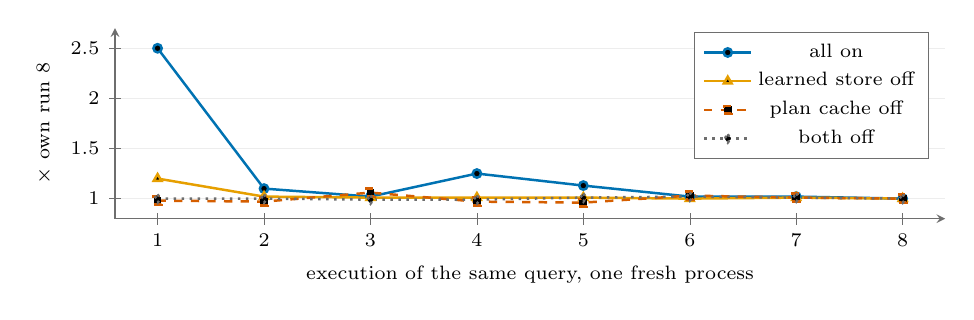
\begin{tikzpicture}
\begin{axis}[
  width=\columnwidth, height=40mm,
  xmin=0.6, xmax=8.4, ymin=0.8, ymax=2.7,
  xtick={1,2,3,4,5,6,7,8}, ytick={1.0,1.5,2.0,2.5},
  axis lines=left, axis line style={draw=pfigGray},
  ymajorgrids, grid style={pfigLight, line width=0.4pt},
  tick style={draw=pfigGray},
  xlabel={execution of the same query, one fresh process},
  ylabel={$\times$ own run 8},
  xlabel style={font=\scriptsize}, ylabel style={font=\scriptsize},
  xticklabel style={font=\scriptsize}, yticklabel style={font=\scriptsize},
  legend style={font=\scriptsize, draw=pfigGray, at={(0.98,0.98)},
                anchor=north east, legend columns=1},
]
\addplot[draw=okBlue, mark=*, mark size=1.5pt, line width=0.9pt]
  coordinates {(1,2.50) (2,1.10) (3,1.02) (4,1.25) (5,1.13) (6,1.02) (7,1.02) (8,1.00)};
\addlegendentry{all on}
\addplot[draw=okOrange, mark=triangle*, mark size=1.6pt, line width=0.9pt]
  coordinates {(1,1.20) (2,1.02) (3,1.01) (4,1.01) (5,1.01) (6,1.00) (7,1.01) (8,1.00)};
\addlegendentry{learned store off}
\addplot[draw=okVermillion, mark=square*, mark size=1.4pt, dashed, line width=0.9pt]
  coordinates {(1,0.98) (2,0.97) (3,1.06) (4,0.97) (5,0.96) (6,1.03) (7,1.01) (8,1.00)};
\addlegendentry{plan cache off}
\addplot[draw=pfigGray, mark=diamond*, mark size=1.5pt, dotted, line width=0.9pt]
  coordinates {(1,1.00) (2,1.00) (3,0.99) (4,0.99) (5,1.01) (6,1.02) (7,1.01) (8,1.00)};
\addlegendentry{both off}
\end{axis}
\end{tikzpicture}
\caption{\E{11}: four-arm ablation, TPC-H sf1, round r4 (load 0.3 per core); geometric mean over
22 queries of each execution's time over the same arm's eighth. Each curve is normalized to
itself, so it shows what repetition gains, not which arm is faster; the learned-store-off arms
are about $4$ to $10\times$ slower in absolute terms because they recompute column statistics.}
\label{fig:learning}
\end{figure}

A second execution is faster for many reasons, so a before-and-after comparison cannot
establish a learning loop. \E{11} runs each TPC-H query eight times in a fresh process under
four configurations (everything on, plan cache off, learned store off, both off), normalizing
each curve to its own steady state. \Cref{fig:learning} shows the round that started on the
quietest box, and three other rounds agree on its shape. With everything on, the first execution
costs $2.50\times$ the steady state (2.64 and 2.77 in two other rounds); with the plan cache
off, $0.98$. \emph{The plan cache accounts for the whole first-to-steady improvement on repeated
TPC-H queries}, and nothing here shows measured row counts making a later execution faster.
With the learned store off and the plan cache on, the curve is $1.2\times$, but that arm also
stops caching per-column statistics across queries, which alone raises steady-state time from
about 16\,ms to about 150\,ms a query. The store's measurable value on this workload is
therefore statistics reuse. The experiment cannot separate execution feedback from it, and a
switch that isolates the feedback path is the next measurement. These runs predate the fix that
files an aggregate's measured count where the estimator reads it (\cref{sec:learning}).

\subsection{Scale-out}
\label{sec:eval-cluster}

\begin{table}[tbp]
\centering\footnotesize
\setlength{\tabcolsep}{3.0pt}
\begin{tabular}{@{}lrrrrr@{}}
\toprule
Pipeline & \sys{} & Ray Data & Daft & vs Ray & vs Daft \\
\midrule
filter, count & 282\,ms & 2{,}902\,ms & 1{,}701\,ms & \win \textbf{10.3}$\times$ & \win \textbf{6.0}$\times$ \\
\texttt{group\_by} & 322\,ms & \emph{t/o} & 1{,}200\,ms & --- & \win \textbf{3.7}$\times$ \\
\texttt{join} & 1{,}845\,ms & \emph{t/o} & 201{,}165\,ms & --- & \win \textbf{109}$\times$ \\
UDF map & 744\,ms & \emph{t/o} & \emph{err} & --- & --- \\
\bottomrule
\end{tabular}
\caption{\E{7}: TPC-H sf100 Parquet on S3; 100 four-CPU workers plus a head with no worker CPU;
engines run sequentially (\sys{}, Ray Data, Daft), best of two, 400\,s timeout; result
signatures compared across engines before a timing is kept. \emph{t/o} (timeout) and
\emph{err} (engine error) get no ratio and mean the engine did not finish this experiment, not
that it cannot express the pipeline. \sys{}'s mean fleet CPU utilization ranged 17\% to 60\% by
pipeline. Excluded: \texttt{scan\_count}, which \sys{} answers from Parquet footers in 2\,ms, a
better plan rather than distributed throughput.}
\label{tab:cluster}
\end{table}

At sf100 (\E{7}), \sys{} leads Daft on every pipeline that produced a number, and Ray Data did
not finish three of the four inside the timeout. Engines ran in a fixed, unrandomized order on
shared object storage, so a later engine could see a warmer bucket. An earlier round put \sys{}
behind, with every cause in the control plane and none in an operator: a derived worker count
read as a user override suppressed the cluster fill, any stage containing a UDF fell back to the
single-node orchestrator, and a join reducer sent 3.75M rows back through Python. On a separate 16-node fleet of 8-CPU workers reading TPC-H from S3 (2026-07-12), \sys{}
led Daft $1.72$ to $2.23\times$ on \texttt{join} across sf1, sf10 and sf100 and trailed it at
$0.84\times$ on the storage-bound \texttt{filter\_count} at sf100. Two fleet sizes on different
workloads do not make a scaling curve, and \sys{} has not measured one.

\subsection{Worker loss}
\label{sec:eval-dist}

\begin{table}[tbp]
\centering\footnotesize
\setlength{\tabcolsep}{3.0pt}
\begin{tabular}{@{}lrrrl@{}}
\toprule
Arm & ms & vs $r{=}1$ & vs own & Result \\
\midrule
no fault, $r{=}1$              & 258.0 & 1.00$\times$ & 1.00$\times$ & \win equivalent \\
no fault, $r{=}2$              & 172.7 & 0.67$\times$ & 1.00$\times$ & \win equivalent \\
1 lost at reduce, $r{=}1$      & 733.6 & 2.84$\times$ & 2.84$\times$ & \win equivalent \\
1 lost at reduce, $r{=}2$      & 2167.1 & \loss 8.40$\times$ & \loss 12.55$\times$ & \win equivalent \\
2 lost at reduce, $r{=}2$      & 2215.4 & \loss 8.59$\times$ & \loss 12.83$\times$ & \win equivalent \\
1 lost during map              & 1723.1 & 6.68$\times$ & 6.68$\times$ & \win equivalent \\
2 lost during map              & 1755.7 & 6.81$\times$ & 6.81$\times$ & \win equivalent \\
\bottomrule
\end{tabular}
\caption{\E{8}: five injected worker-loss arms and two no-fault controls on a grouped aggregate
over 8M rows and 5{,}000 keys, 8 workers on one machine; $r$ is the shuffle replication factor.
A worker lost \emph{at reduce} has already published its buckets, which vanish with it; one lost
\emph{during map} has published nothing, and its split is relocated. \emph{vs $r{=}1$} is the cost
against the default configuration, \emph{vs own} the cost to a deployment already running with
replicas.}
\label{tab:faults}
\end{table}

All five fault arms return a relation equivalent to the single-node answer (\cref{tab:faults}),
which is the purpose of \cref{eq:merge} and the protocol of \cref{sec:recovery}, here tested
against killed workers instead of generated partitionings. Losing two workers cost about what
losing one did, in both phases. Independent partials permit parallel regeneration, but the
totals cannot show it: a fixed detection timeout would produce the same shape, and \E{8}
recorded no per-phase trace. Replication did not pay. Copying every published bucket to a
survivor turned a $2.84\times$ recompute into an $8.40\times$ recovery. Replication assumes that
re-reading a source from object storage is expensive, which is false on one machine with an
in-memory source, so this run measures its fixed cost and not its benefit.

\subsection{GPU and model pipelines}
\label{sec:eval-gpu}

\begin{table*}[tbp]
\centering\footnotesize
\setlength{\tabcolsep}{3.6pt}
\begin{tabular}{@{}lllrrl@{}}
\toprule
Workload & Model (weights) & Input and batch size & Rate & GPU busy & Unit \\
\midrule
Image classification, fused & ResNet-50 (random init) & 131{,}072 JPEGs; 128 & 2{,}576 & 78\% & images/s \\
Decode $+$ infer, two stages & ResNet-50 (random init) & 131{,}072 JPEGs; 128 & 2{,}504 & 81\% & images/s \\
Image embeddings, 2048-d & ResNet-50 features (random init) & 12{,}000 images; 256 & 2{,}502 & 80\% & images/s \\
Zero-configuration & ResNet-50 (random init) & 131{,}072 JPEGs; engine default & 2{,}451 & 82\% & images/s \\
Two models per GPU & EfficientNet-B0 (random init) & 49{,}000 images; \texttt{num\_gpus=0.5} & 6{,}764 & 89\% & images/s \\
Video clips, per-frame & ResNet-18 (random init) & 4{,}096 16-frame clips; 64 & 2{,}075 & --- & clips/s \\
Audio features & mel on CPU, ResNet-18 & 16{,}384 clips; 128 & 38{,}546 & --- & clips/s \\
Text embeddings, 384-d & all-MiniLM-L6-v2 (pretrained) & 8{,}192 texts; 256 & 33{,}611 & --- & texts/s \\
LLM generation & gpt2 FP16 (pretrained), greedy & 2{,}048 prompts; 32; 32 new tokens & 815 & --- & prompts/s \\
Image generation & DDPM CIFAR-10 (pretrained), 20 DDIM steps & 2{,}048 images; 64 & 169 & --- & images/s \\
Training ingest & none (\texttt{iter\_torch\_batches}) & 200{,}000 rows, 1024-d; 256 & 1.06M & --- & rows/s \\
\bottomrule
\end{tabular}
\caption{\E{10}: eleven GPU workloads on 8$\times$T4, each an operator in an ordinary plan gated
on agreement with a single-process reference; seven distinct models, the ResNet-50 rows sharing
one network. All rows but zero-configuration pass the batch size shown. \emph{GPU busy} is NVML's
utilization counter (fraction of time a kernel was executing), sampled every 0.25\,s per device,
averaged, and recorded on five rows only; it says nothing about occupancy or achieved FLOPs.
Torchvision networks are randomly initialized under a fixed seed: the same kernels as trained
weights, but prediction agreement then checks determinism, not accuracy.}
\label{tab:gpu}
\end{table*}

\Cref{tab:gpu} reports coverage only, across images, video, audio, text and generation. The
zero-configuration row carries the interface claim. With no batch size,
\texttt{ds.map\_batches(Model, num\_gpus=1)} ran at 2{,}451 images/s against 2{,}504 with
\texttt{batch\_size=128}, 2.1\% slower, because the engine derives a default from row width and
free device memory, overlaps decode with the forward pass, and halves a batch on an
out-of-memory error. That is one model at one row width, and \sys{} has not published a batch-size
sweep against it.

Head-to-head, three results hold and two go the other way. All ran \sys{} under its default FP16
autocast and the comparators at their default precision (FP32 for the torch workloads), so they
compare defaults, not equal numerical work.

\textbf{Image scoring} (\E{9}): six single-T4 nodes, 100{,}000 small JPEGs on S3, and a
dense-matrix scorer in cupy that every engine built identically, not a trained vision model.
\sys{} finished in 18.72\,s against Ray Data's 44.19 and Daft's 101.10 ($2.36\times$ and
$5.40\times$), with checksums agreeing within 0.15\%, the JPEG decoders' difference. The scorer
is 15\% of \sys{}'s time, so the margin lies in object reads and decode, and in scheduling.

\textbf{LLM generation} (\E{10}): gpt2, greedy decoding, 32 new tokens per prompt, 65{,}536
prompts of 10 to 20 tokens. \sys{} produced identical text at 1{,}521 prompts/s against Ray
Data's 227, $6.71\times$. At 32{,}768 prompts the ratio was $13.4\times$, but Ray Data's rate was
still rising with scale, so the larger run is the better estimate and a larger one might read
lower again. Scale cut the text-embedding ratio likewise, from $29.5\times$ at 8{,}192 texts to
$1.52\times$ at 1.3 million, where \sys{}'s rate was flat and Ray Data's had caught up. A ratio
taken while the slower engine is still amortizing its start-up measures the start-up.

\textbf{Compute-bound inference} crosses over with size: $8.6\times$ at 125{,}000 rows,
$2.5\times$ at 500{,}000, $0.96\times$ at two million, $0.76\times$ at four. The cause is that a
fused CPU-then-GPU map runs \sys{}'s CPU stage in threads inside the device-holding actors and
Ray Data's in processes. A factor there means nothing without its row count.

\textbf{Two-stage decode-then-infer} over 131{,}072 JPEGs goes the other way: $0.85\times$ Ray
Data (2{,}007 against 2{,}373 images/s, identical predictions). Ray Data's devices are 80\% busy at
297 images/s per T4, near the 285 the same T4s reach fused; \sys{}'s are 73\% busy, and the loss
is device idle time in the hand-off. Sweeping decode concurrency and the credit window moved it under
3\%. Double-buffering the terminal consumer reached 2{,}232 images/s at 80\% busy but was
reverted, because the autoscaler read the emptied queue as over-provisioning and halved the
worker pool on the one-stage benchmark.

\textbf{29\,GB batch inference} over 200{,}000 images measured $1.51\times$ Ray Data once. Later
runs, after cluster nodes had begun dropping out under sustained load, gave \sys{} 989 to
1{,}666 images/s against Ray Data's steady 1{,}506 to 1{,}621. We report it as unreproduced. An
earlier $0.42\times$ came from two read-path defects, a \texttt{uint8} tensor widened to
\texttt{int64} at the FFI boundary and the row-count read batch of \cref{sec:memory}. Fixing both
cut a single-node reproduction's peak RSS from 11.47\,GB to 3.09\,GB.

% ===========================================================================
\section{Limitations and threats to validity}
\label{sec:limitations}
% ===========================================================================

The experiments span several workload classes and establish no uniform superiority.
\Cref{tab:matrix} gives the support matrix with evidence per cell; \cref{sec:appendix-status}
separates what is evaluated here from what is only implemented.

\emph{Storage is the largest open gap.} \sys{} owns no storage format and decodes dictionaries
at the leaf, which costs it the string and zone-map cases of \cref{sec:eval-storage} and the
sf10-from-Parquet result of \cref{sec:eval-tpch}. The fix lies in the reader, the boundary and
the type system, not in a kernel.

\emph{Streaming is micro-batch and falls short of Flink's guarantees.} \sys{} has no persistent
operator graph, barrier protocol or keyed state backend with point lookups, and its driver is a
single point of failure with no standby. Exactly-once output holds for the sinks of
\cref{sec:streaming} under a single writer. Two concurrent queries writing one table are not
coordinated. A worker lost mid-trigger makes the driver restart the trigger from its checkpoint.
Unit tests inject failures on that path and crash-and-restart tests interrupt every point of the
commit sequence, but no test yet kills a real worker during a distributed micro-batch.

\emph{Distributed coverage has holes.} An inequality join scales only by broadcasting its right
side. Several global window functions refuse to distribute, and a plan gets one CPU-to-GPU
resource boundary. Recovery was tested only with a surviving driver and on one machine, and complete
pipelines have no node-count scaling curve (\cref{sec:eval-cluster,sec:eval-dist}).

\emph{Continuous integration checks the device tier by type, not by value.} CI installs neither
Ray nor a GPU. The distributed and GPU results rest on recorded runs at the revisions
\cref{tab:protocol} dates, and until one is repeated, later changes on those paths are covered
only by the schema contract and the pandas-backed translation tests.

\emph{Threats to validity.} \emph{Best of $N$, warm}: \E{1} reports the minimum of five runs of
the same query, a shape a memoizing engine wins, and \sys{}'s session carries a plan cache and
learned store across those repeats where DuckDB and Polars have neither. \E{11} puts the plan
cache at about $2.5\times$ on a repeated TPC-H query, so a warm best-of-five favours \sys{}.
\E{12} gives the spread, not a cold comparison. \emph{Correctness gate}: a case \sys{} fails
leaves its geometric mean, which can flatter the aggregate, so \E{12} reports requested, correct
and timed counts per engine. \emph{Timed path}: the gate precedes the timed repetitions, between
which adaptive strategies can change. Each strategy is result-equivalent by construction and
separately covered by the oracle tests, but the timed physical plan is not re-checked.
\emph{Precision}: the GPU head-to-heads pit \sys{}'s FP16 default against the torch
comparators' FP32. \emph{Comparator configuration}: we found and fixed an adapter defect that
left Ray Data with one of 96 cores, three Spark adapter defects, and a Daft startup timeout
shorter than the fleet's first-use environment build. Others may remain.

% ===========================================================================
\section{Related work}
\label{sec:related}
% ===========================================================================

\paragraph{Vectorized and compiled single-node execution.} Columnar batch-at-a-time execution
begins with MonetDB/X100~\cite{boncz2005monetdb}, compiled execution with
HyPer~\cite{neumann2011compiling}; Umbra~\cite{neumann2020umbra} contributed the inline-prefix
string representation \cref{sec:eval-storage} names as a gap here. \sys{} is
morsel-driven~\cite{leis2014morsel} and vectorized, with a Cranelift-compiled
path~\cite{cranelift}; DuckDB~\cite{raasveldt2019duckdb} is its closest single-node comparator.
Velox~\cite{pedreira2022velox} and DataFusion~\cite{lamb2024datafusion} are embeddable engines
that leave distribution to a host. DataFusion shares Rust, Arrow and much of the operator set
with \sys{}. Its execution-plan trait admits any operator implementing it, so a mergeable form
is available but not required. Photon~\cite{behm2022photon} is a vectorized engine inside a
lakehouse runtime rather than an embeddable library.

\paragraph{Distributed dataflow and warehouses.} The mergeable triple comes from MapReduce's
combiner~\cite{dean2004mapreduce} and Gray et al.'s algebraic aggregates~\cite{gray1997datacube};
the contribution here is refusing any stateful operator that declares no contract.
Spark~\cite{zaharia2012rdd,armbrust2015sparksql} runs local and cluster modes through the same
physical operators, with binary memory management and whole-stage code generation, and its
adaptive execution re-plans at shuffle boundaries~\cite{sparkaqe}. \sys{}'s \Cb{} contract
follows Volcano's separation of operators from exchange~\cite{graefe1994volcano}. Cloud
warehouses~\cite{sethi2019presto,dageville2016snowflake} answer the same questions as a service,
not a library, and \sys{}'s transactional sinks write the lakehouse
formats~\cite{armbrust2020delta}.

\paragraph{Streaming and unified execution.} \sys{}'s micro-batch path adopts Structured
Streaming's unbounded-table framing~\cite{armbrust2018structured}.
Summingbird~\cite{boykin2014summingbird} made the monoid the unifying abstraction so one program
compiles to a batch and an online engine, and the Dataflow model~\cite{akidau2015dataflow} gave
the two one specification, whose \texttt{CombineFn} has the shape of \Ca{}. Both unify the
program above engines; \sys{} makes the contract the admission test for one engine's operators.
Flink~\cite{carbone2015flink}, a single runtime treating bounded input as a special case, has
what \sys{} lacks: a persistent operator graph, barrier snapshots and a keyed state backend.
Naiad~\cite{murray2013naiad} is another single-dataflow answer. DBSP~\cite{budiu2023dbsp}
derives incremental operators from a query algebra with signed updates, expressing removals
\sys{}'s partial log cannot.

\paragraph{Adaptive and learned optimization.} Estimation begins with
Selinger~\cite{selinger1979access}. Stage-boundary re-planning descends from
eddies~\cite{avnur2000eddies} and mid-query re-optimization; Spark AQE is its closest deployed
relative at the same grain. Learned optimizers~\cite{marcus2019neo,marcus2021bao,kipf2019learned}
use models to choose which plan runs. Bao steers a validated optimizer with hints instead of
replacing it, so it differs from \sys{} in the size of the decision a model makes, not in
answer correctness. \sys{} takes a lighter route, with
sketches~\cite{flajolet2007hyperloglog,cormode2005countmin}, refit cost coefficients and a
bandit~\cite{auer2002ucb} over result-equivalent strategies: its cold start is the untuned
system, and it gives up correcting a badly wrong plan. Leis et al.~\cite{leis2015goodjoin}
supply both the standing argument for measured cardinalities and the benchmark \sys{} still
loses.

\paragraph{Data systems for machine learning.} The model evaluation is measured against
Ray~\cite{moritz2018ray} and Ray Data~\cite{luan2025streamingbatch}, the closest system to
\cref{sec:gpu}. Daft~\cite{daft} is the closest multimodal relational engine; its documentation
describes cost-based join reordering and multimodal-aware scheduling, so a comparison must name
a release. We compare relational and inference pipelines against Daft 0.7.24 but have not run a
full mixed relational-and-model pipeline on it. \sys{}'s computed epoch permutation comes from
MosaicML's StreamingDataset~\cite{mosaicstreaming}. NoScope~\cite{kang2017noscope} and
BlazeIt~\cite{kang2020blazeit} put a model inside the optimizer, approximating with cascades,
proxy models and control variates where the semantics allow; for their target queries those
techniques are stronger than anything here. \sys{} makes decode, embedding and inference
ordinary expressions and approximates nothing.

% ===========================================================================
\section{Conclusion}
% ===========================================================================

The evaluation supports a narrower claim than ``one engine wins''. On named single-node suites
\sys{} is faster than DuckDB over identical Arrow input and competitive with DuckDB's own
storage, using about twice the CPU for its latency. On one 100-worker fleet it finishes TPC-H
pipelines Ray Data did not and leads Daft on the rest. It loses the Join Order Benchmark and
sf10 read from Parquet, trails Ray Data on a two-stage GPU pipeline, and has a weaker streaming
path than a Flink-class system. Its repeated-query speedup comes from a plan cache any engine
could add, not from the learning loop.

\sys{} tests one design rule: a stateful operator enters the engine only with a declared
execution contract, and the scheduler dispatches on nothing else. Three contracts cover the
whole vocabulary once the second is read as partition-local evaluation and the third as
replicate-or-iterate under a budget, and a registry with an exhaustive test keeps a new operator
from skipping the classification. Stating the contracts precisely forced several repairs to the
engine, each to code that had passed every test: integer \texttt{SUM} overflow that depended
on the partition count, a shuffle that could return a short relation when a bucket went missing,
a checkpoint policy whose write bound was false, a learned-cardinality path that filed every
measurement where nothing read it, a transport that could not carry a single batch over 4\,MiB,
and shuffle files that a straggler's backup could truncate while a reducer read them. The last
surfaced only when the paper's own equivalence experiment was rerun with a lever that moved. The part of the hypothesis that matters most for the design remains untested:
whether the contracts survive richer physical representations (dictionary strings, a keyed state
backend) without a fourth contract or a second implementation creeping back in.

{\scriptsize
\setlength{\bibsep}{0pt plus 0.1ex}
\bibliographystyle{abbrvnat}
\bibliography{refs}
}


\appendix
\small
% ===========================================================================
\section{Support matrix and claim ledger}
\label{sec:appendix-matrix}\label{sec:appendix-claims}
% ===========================================================================

\Cref{tab:matrix} states what one engine covers by execution regime (``batch'' includes
morsel-parallel execution on one node), with the evidence for each row; \sys{} claims nothing
marked \emph{no}. \Cref{tab:claims} pairs each claim with its observation and what that
observation does not rule out.

\begin{table}[tb]
\centering\scriptsize
\setlength{\tabcolsep}{2.2pt}
\begin{tabular}{@{}>{\raggedright\arraybackslash}p{0.35\columnwidth}lll>{\raggedright\arraybackslash}p{0.16\columnwidth}@{}}
\toprule
Property & batch & micro-batch & distributed & evidence \\
\midrule
Relation equal under \cref{sec:equivalence} & yes & yes & yes & matrix; \E{3} \\
Float aggregates bit-identical across modes & no & no & no & reassociation \\
Float aggregates bit-identical, same mode and partitioning & yes & yes & yes & oracle tests \\
Integer \texttt{SUM} error independent of partitioning & yes & yes & yes & unit $+$ diff.\ tests \\
Unordered \texttt{LIMIT}, tied \texttt{row\_number}, \texttt{array\_agg} order & open & open & open & subset / rank-set checks \\
\midrule
Event-time windows; late rows dropped and counted & n/a & yes & yes & tests \\
Watermark barriers, retractions, keyed state backend & n/a & no & no & --- \\
Exactly-once: Delta, file, keyed DB & n/a & yes & yes & replay tests \\
Exactly-once: Iceberg & n/a & yes & refused & replay tests \\
Exactly-once: unkeyed DB append; driver failover & n/a & no & no & --- \\
\midrule
Worker-loss recovery, batch shuffle & n/a & n/a & yes & \E{8}; fault tests \\
Worker-loss recovery, mid-trigger & n/a & restart & restart & injected-failure tests \\
Inequality join & yes & --- & replicate or raise & tests \\
Recursive CTE (linear) & yes & --- & iterate, capped & diff.\ tests \\
Spill: agg, distinct, sort, join, window & yes & partial & yes & spill tests \\
CPU$\rightarrow$GPU boundaries & \multicolumn{3}{c}{one per plan} & \E{10} \\
\bottomrule
\end{tabular}
\caption{Support by execution regime, with the evidence for each row. \emph{Open} marks a choice
SQL leaves open (\cref{sec:equivalence}); \texttt{order\_by} closes each. \emph{Partial} spill:
the windowed streaming aggregate spills closed windows and the unwatermarked one raises at its
state ceiling. \emph{Restart}: the trigger is re-run from its checkpoint.}
\label{tab:matrix}
\end{table}

\begin{table}[tb]
\centering\scriptsize
\setlength{\tabcolsep}{2.2pt}
\begin{tabular}{@{}>{\raggedright\arraybackslash}p{0.30\columnwidth}>{\raggedright\arraybackslash}p{0.33\columnwidth}>{\raggedright\arraybackslash}p{0.31\columnwidth}@{}}
\toprule
Claim & Observation & Not excluded \\
\midrule
Partition count changes scheduling, not the relation & property test, mode matrix, \E{3} (2 workers), \E{8} & untested operator combinations; tests, not proof \\
\addlinespace[1pt]
Every stateful operator has a contract & registry test over the IR enums & a contract classified wrongly by hand \\
\addlinespace[1pt]
Buffering memory independent of input size & counting-allocator test: 1\,MB at 1M and 4M rows & high-fan-out operators; receive side scales with peers \\
\addlinespace[1pt]
Faster than DuckDB on identical Arrow & \E{1} six suites; \E{12} intervals & warm, best-of-5, plan cache \\
\addlinespace[1pt]
Leads Daft and Ray Data at sf100 & \E{7}, one fleet size & fixed engine order; no scaling curve \\
\addlinespace[1pt]
Correct under worker loss & \E{8}, five arms & one machine; driver loss \\
\addlinespace[1pt]
Repeated queries get faster & \E{11}: all of it is the plan cache & a benefit from measured row counts, untested \\
\addlinespace[1pt]
The learned store reuses column statistics & \E{11}: 4--10$\times$ steady-state cost without it & one workload \\
\addlinespace[1pt]
Eleven GPU workloads run as plan operators & \E{10}, gated on agreement & random-init weights; five rows sampled for utilization \\
\bottomrule
\end{tabular}
\caption{Claim ledger: each claim with its supporting observation and what that observation
does not rule out.}
\label{tab:claims}
\end{table}

% ===========================================================================
\section{Implementation status}
\label{sec:appendix-status}
% ===========================================================================

\emph{Evaluated here}: contract dispatch and registry; the streaming executor; the Flight
shuffle with byte-weighted credits and completeness manifests; replication and recovery; the
plan cache and statistics reuse; the micro-batch driver, its checkpoints and transactional
sinks; the CPU-to-GPU split; inference and media expressions. \emph{Implemented, not evaluated
here}: the measured-cardinality loop since its fix; the strategy bandit's gain; the cuDF device
tier; spot-preemption migration; partition-aligned operators; lakehouse \texttt{MERGE} and CDC;
governance rewrites. \emph{Open defects}: device idle time in the two-stage GPU pipeline; the
unreproduced 29\,GB run; TPC-H q15, which failed once on a multi-node cluster (``no surviving
worker to recover the join shuffle on'') and has not reproduced locally. \emph{Future work}: dictionary and string-view kernels; a logical/physical type split;
a keyed streaming state backend; driver failover; multi-stage heterogeneous scheduling; a
partitioned inequality join.

% ===========================================================================
\section{Reproducing the results}
\label{sec:appendix-protocol}
% ===========================================================================

\paragraph{Versions.} DuckDB 1.5.5, Polars 1.36.1, Daft 0.7.24, Ray 2.58.0, PySpark 4.2.0,
PyArrow 19.0.1. GPU workers: torch 2.9.1+cu128, cupy 14.2, cuDF 26.06, numpy 2.2.6, Tesla T4,
driver 580.126.20; model checkpoints are not revision-pinned.

\paragraph{Commands} (\texttt{B} is \texttt{benchmarks}; $\langle s\rangle$ a suite).
{\scriptsize\raggedright
\E{1}, \E{12}: \texttt{python B/run.py -{}-benchmark $\langle s\rangle$ -{}-engines batcher,duckdb,duckdb\_arrow,polars -{}-isolate [-{}-repeat 5 -{}-json-out F]}.
\E{2}: \texttt{-{}-benchmark tpch -{}-scale 10}, \texttt{tpcds} or \texttt{job}, \texttt{-{}-engines batcher,duckdb}.
\E{3}: \texttt{python B/scenarios/claims/scheduler\_equivalence.py -{}-num-workers 2 -{}-source D}.
\E{4}, \E{5}: \texttt{B/scenarios/claims/cost\_bench.py}, \texttt{cold\_start.py}.
\E{11}: \texttt{B/scenarios/claims/learning\_curve.py -{}-runs 8 -{}-arm A}.
\E{6}: \texttt{python B/scenarios/streaming\_throughput.py -{}-runs 5}.
\E{7}: \texttt{BENCH\_ENGINE\_TIMEOUT=400 python B/cluster/vs\_ray\_daft.py 100}.
\E{8}: \texttt{python B/cluster/robustness/worker\_loss.py -{}-rows 8000000 -{}-keys 5000 -{}-workers 8 -{}-rounds 3}.
\E{9}, \E{10}: \texttt{B/gpu\_backend/vs\_ray\_daft\_gpu\_inference.py}, \texttt{B/cluster/gpu\_*.py}.\par}

\paragraph{Identity, gate and artifact.} After an in-place rebuild once swapped the engine
mid-benchmark, the harness now refuses a debug build and records the SHA-256 of
the extension actually loaded before and after each run. The correctness gate has also caught
comparator defects: two engines folded TPC-H q6's \texttt{0.06 + 0.01} bound in IEEE double and
dropped every row with \texttt{l\_discount = 0.07}. The 2026-09-23 raw results are in
\texttt{benchmarks/results/paper\_2026-09-23/}; no content-addressed manifest yet
binds them.

\end{document}
